\section{Desarrollo de Aplicación en Android}

\par 
El desarrollo de la aplicación en Android no requiere de un software especializado como es en el caso de iOS. Solamente es necesario una computadora con un sistema operativo: Windows, Mac Os o Linux. El entorno de desarrollo que utilizaremos es Android Studio; ya que, es soportado oficialmente por Google y recibe actualizaciones habitualmente. Adicional no es indispensable más si es recomendable utilizar un dispositivo de prueba con la versión de Android para cual estaremos desarrollando. Android Studio cuenta con un emulador con capacidad de emular la mayoría de los dispositivos Android en el mercado; sin embargo, dependiendo de qué tan reciente sea el dispositivo que emular, de la misma manera utilizará más recursos del computador.

\clearpage

\par \noindent
Recordemos que el objetivo de la aplicación es el siguiente: establecer una comunicación bluetooth con nuestro prototipo y dependiendo de los parámetros asignados por el usuario final. Capturar las mediciones de temperatura respetando los parámetros seleccionados por el usuario y guardando los resultados en una base de datos local para ser consultados después.

\par \noindent
Nuestra aplicación requiere esencialmente de 3 elementos que debemos desarrollar: 

\begin{itemize}
	\item La interfaz
	\item Los Servicios del segundo plano
	\item La base de datos
\end{itemize}

\par \noindent
Como es necesario primero diseñar la interfaz para poder insertar datos en nuestra aplicación empezaremos por ahí. Cabe a destacar que la compañía SIGCSA nos ha dado el permiso de utilizar los logos y colores oficiales de la compañía para el desarrollo de la aplicación.

\subsection{Interfaz de la Aplicación}

\par
Al inicio de la aplicación mostraremos una animación con el logo y el eslogan de la compañía. El tiempo de duración de esta animación es de 2 segundos y se ejecutara siempre y cuando la aplicación no entre en el segundo plano del sistema operativo. La imagen de la animación es la siguiente:

\begin{figure}[H]
	\centering
	
\includegraphics[width=0.2\linewidth]{interfaz1.png}
	\caption{Animación de inicio de la aplicación; también conocido como "Splash Screen"}
\end{figure}

\par \noindent
Transcurridos los 2 segundos de la animación automáticamente es reemplazado por la actividad principal.  

\subsubsection{Actividad Principal}

\begin{figure}[H]
	\centering
	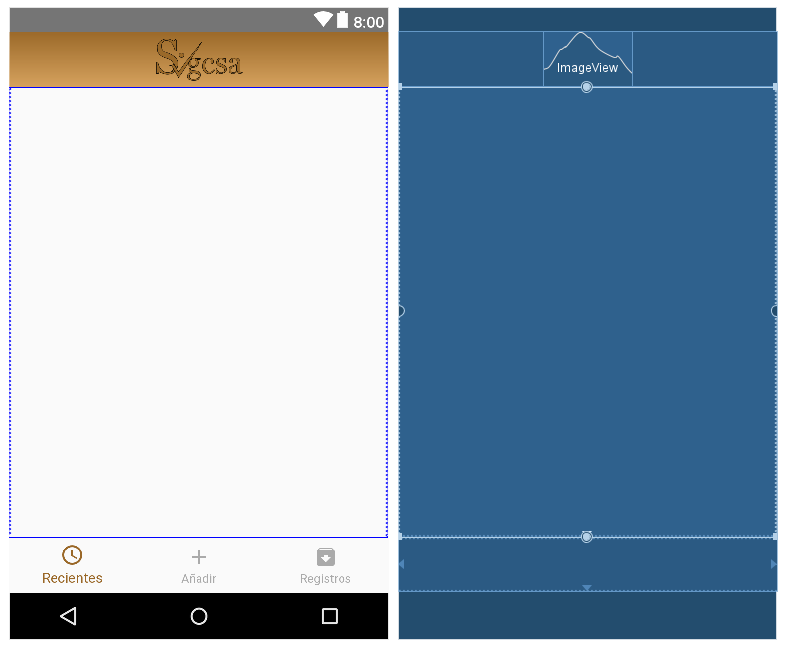
\includegraphics[width=0.8\linewidth]{interfaz2.png}
	\caption{Interfaz de la actividad principal}
\end{figure}

\par 
Pero ¿Qué es una actividad? y ¿Por qué es la actividad principal? Según la documentación oficial de Android una actividad se define como: un componente de aplicación que proporciona una pantalla con la que los usuarios pueden interactuar para hacer algo, como marcar el teléfono, tomar una foto, enviar un correo electrónico o ver un mapa. Una actividad puede iniciar otras actividades, incluidas actividades que viven en aplicaciones separadas.\cite{androidapp}

\par \noindent
Se ha llamado la actividad principal porque es donde el usuario final interactúa con el resto de los componentes de la aplicación tales como menús, actividades, fragmentos y servicios. 

\par \noindent
En la imagen 3.10 podemos apreciar los 3 componentes de la actividad principal. En la parte superior se encuentra el "toolbar", su objetivo es el de mostrar información relativa a la actividad donde se encuentra; por lo que, hemos elegido utilizar el logo de la compañía SIGCSA para enfatizar que es la actividad principal. 

\par \noindent
En la parte inferior nos encontramos con una tendencia en la navegación de la aplicación móviles hoy en día. En Android es llamado "BottomNavigationView", como su nombre lo indica es el encargado del manejo de las distintas fragmentos o subinterfaces utilizadas en una aplicación móvil. Es una cinta con el color de fondo de la aplicación en ella se encuentran botones que incluyen el texto y una pequeña imagen. Al seleccionar uno de estos botones la interfaz cambia con la excepción del "toolbar" y el "BottomNavigationView"; adicional el botón seleccionado incrementa ligeramente su tamaño y toma un color distinto al resto de los botones para indicar la interfaz activa en ese momento.

\par \noindent
El ultimo componente de la interfaz de la actividad principal no es visible para el usuario; sin embargo, se puede ver el borde azul en la imagen 3.10. Este componente es un "layout", en él es donde se pueden colocar otros componentes como botones, texto y más. Actúa realmente como un contenedor de componentes. En la actividad principal se encuentra vacío debido a que al iniciar la actividad debemos reemplazar este "layout" por una subinterfaz o fragmento. Por ende este componente es donde son expuestos los fragmentos seleccionados por el "BottonNavigationView" y nosotros hemos programado que el fragmento por defecto al iniciar esta actividad es el fragmento reciente.

\subsubsection{Fragmento Recientes}

\begin{figure}[H]
	\centering
	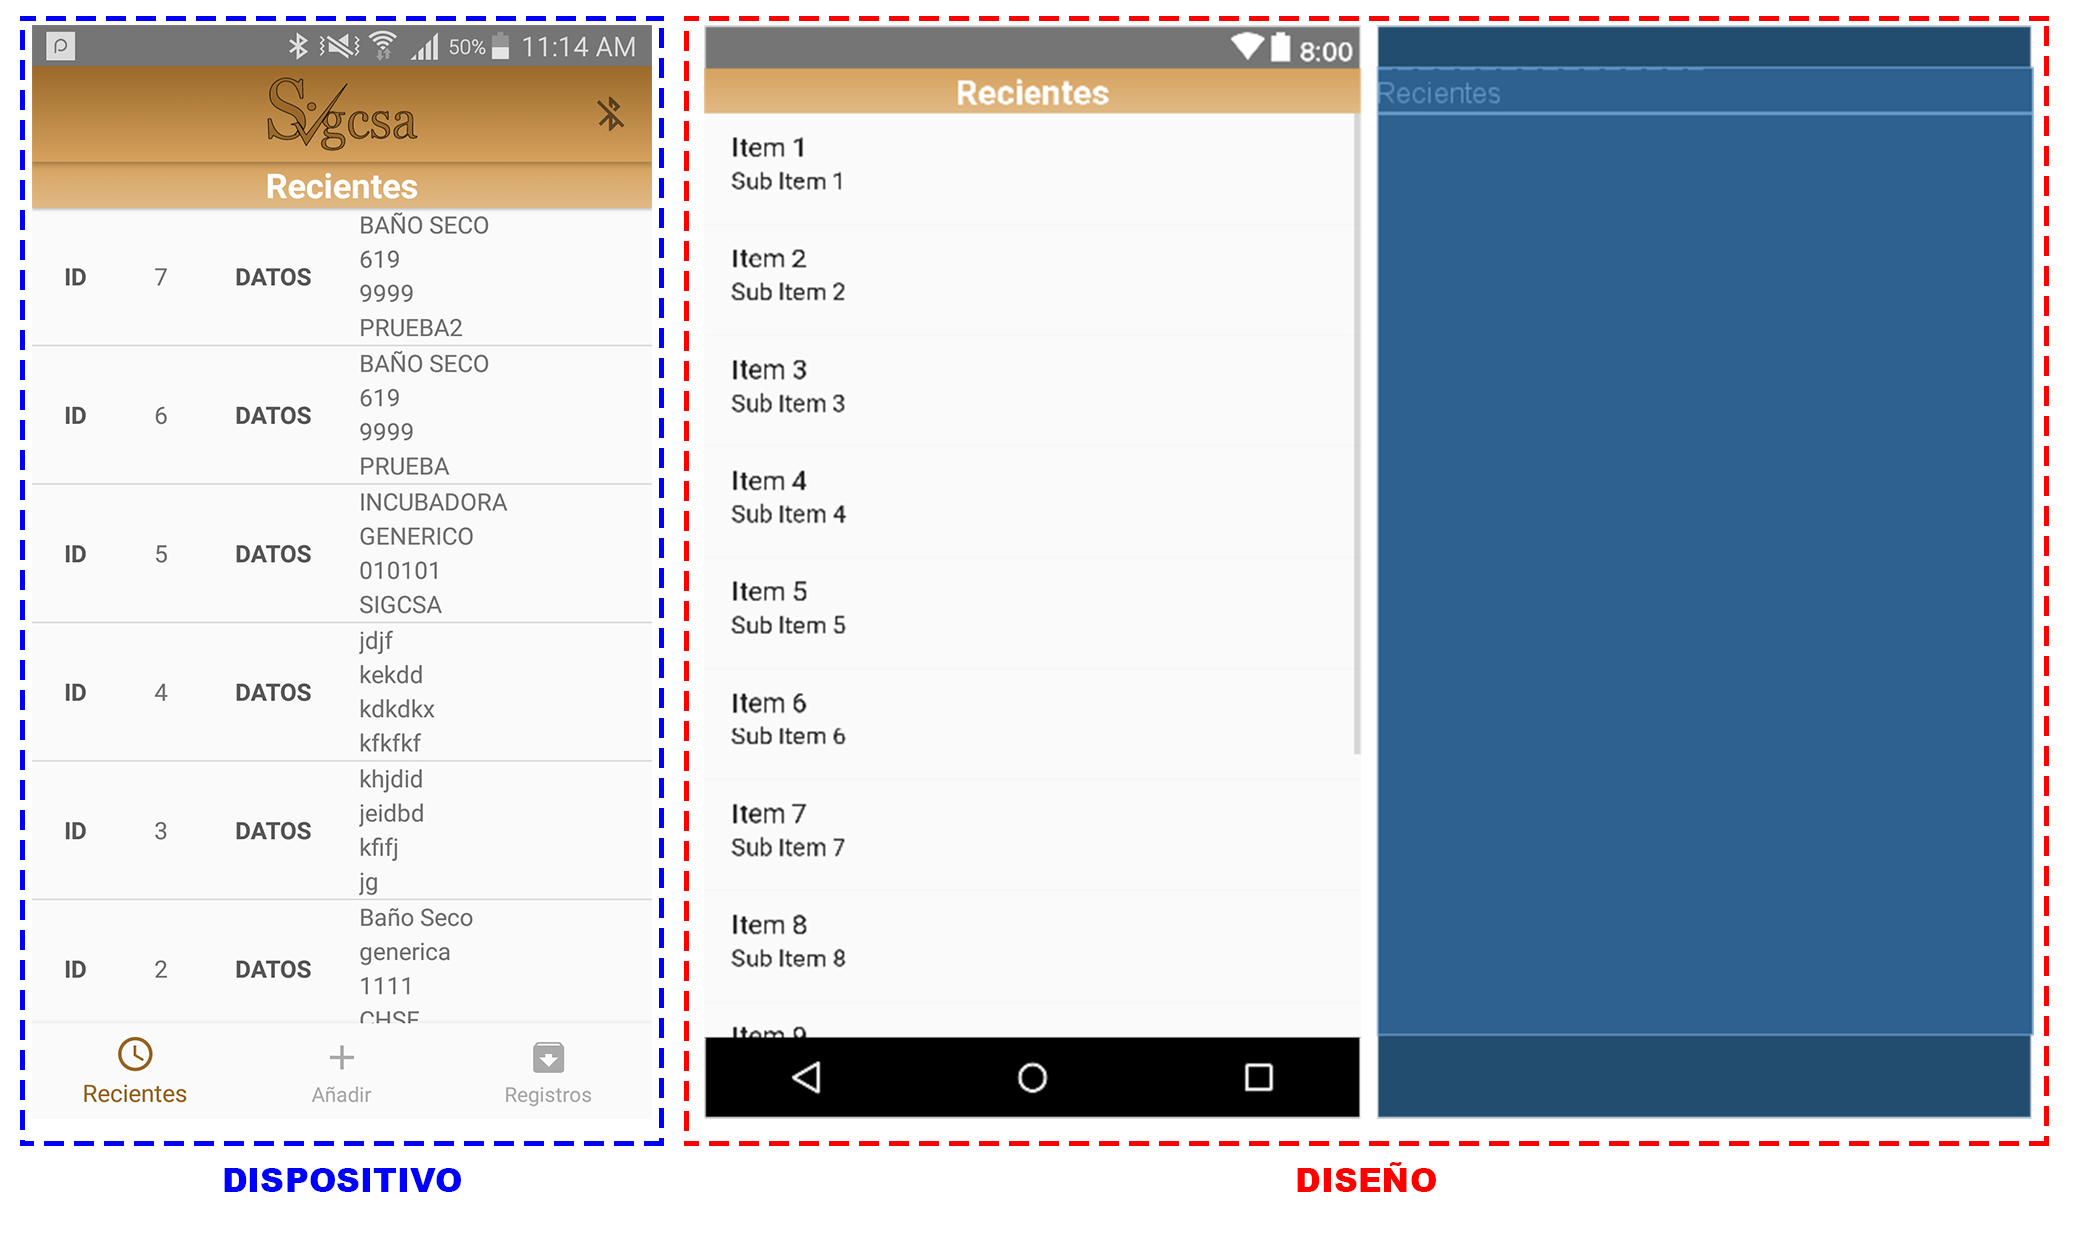
\includegraphics[width=\linewidth]{interfaz3.png}
	\caption{Interfaz del Fragmento Recientes en la aplicación y durante el diseño}
\end{figure}

\par \noindent
Al iniciar la aplicación, se inicia la actividad principal y el valor programado por defecto del "BottonNavegationView" es "Recientes"; por lo que, se procede a visualizar el fragmento reciente en la actividad principal. Un fragmento define una parte distinta del comportamiento de una actividad, incluida la interfaz de usuario asociada. Tiene su propio ciclo de vida que es similar al de la actividad y puede existir junto con otros fragmentos que están integrados en la actividad. Mientras se está ejecutando una actividad, puede agregar y eliminar fragmentos e incluir cada fragmento en una pila posterior administrada por la actividad, lo que permite al usuario navegar hacia atrás a través de los estados de los fragmentos, sin abandonar la actividad\cite{androidapp}. Está compuesto solamente por 3 componentes. 

\par \noindent
El componente principal es el "layout" que contiene los otros dos elementos que hacen la interfaz del usuario. Recordemos que es importante que los elementos de un fragmento se encuentren dentro de un "layout" ya que es más sencillo importar un layout a la actividad principal que todos los componentes por separado. El segundo componente es un "textview" su único objetivo es el de mostrar texto en la aplicación; sin embargo, puede ser utilizado para indicar al usuario partes de la interfaz. El "textview" despliega el texto "Recientes" y tiene un fondo similar al "toolbar" de la aplicación, esto es para brindar uniformidad en los colores de la aplicación. 

\par \noindent
El último elemento es un "ListView" es un componente especial porque podemos agregarle elementos de forma dinámica como una lista, podemos definirle la interfaz de sus elementos y cada elemento de la lista puede actuar como un botón para iniciar otra actividad. Es un elemento muy versátil e indispensable cuando trabajamos con bases de datos o cuando necesitamos ordenar información importante al usuario.

\begin{figure}[H]
	\centering
	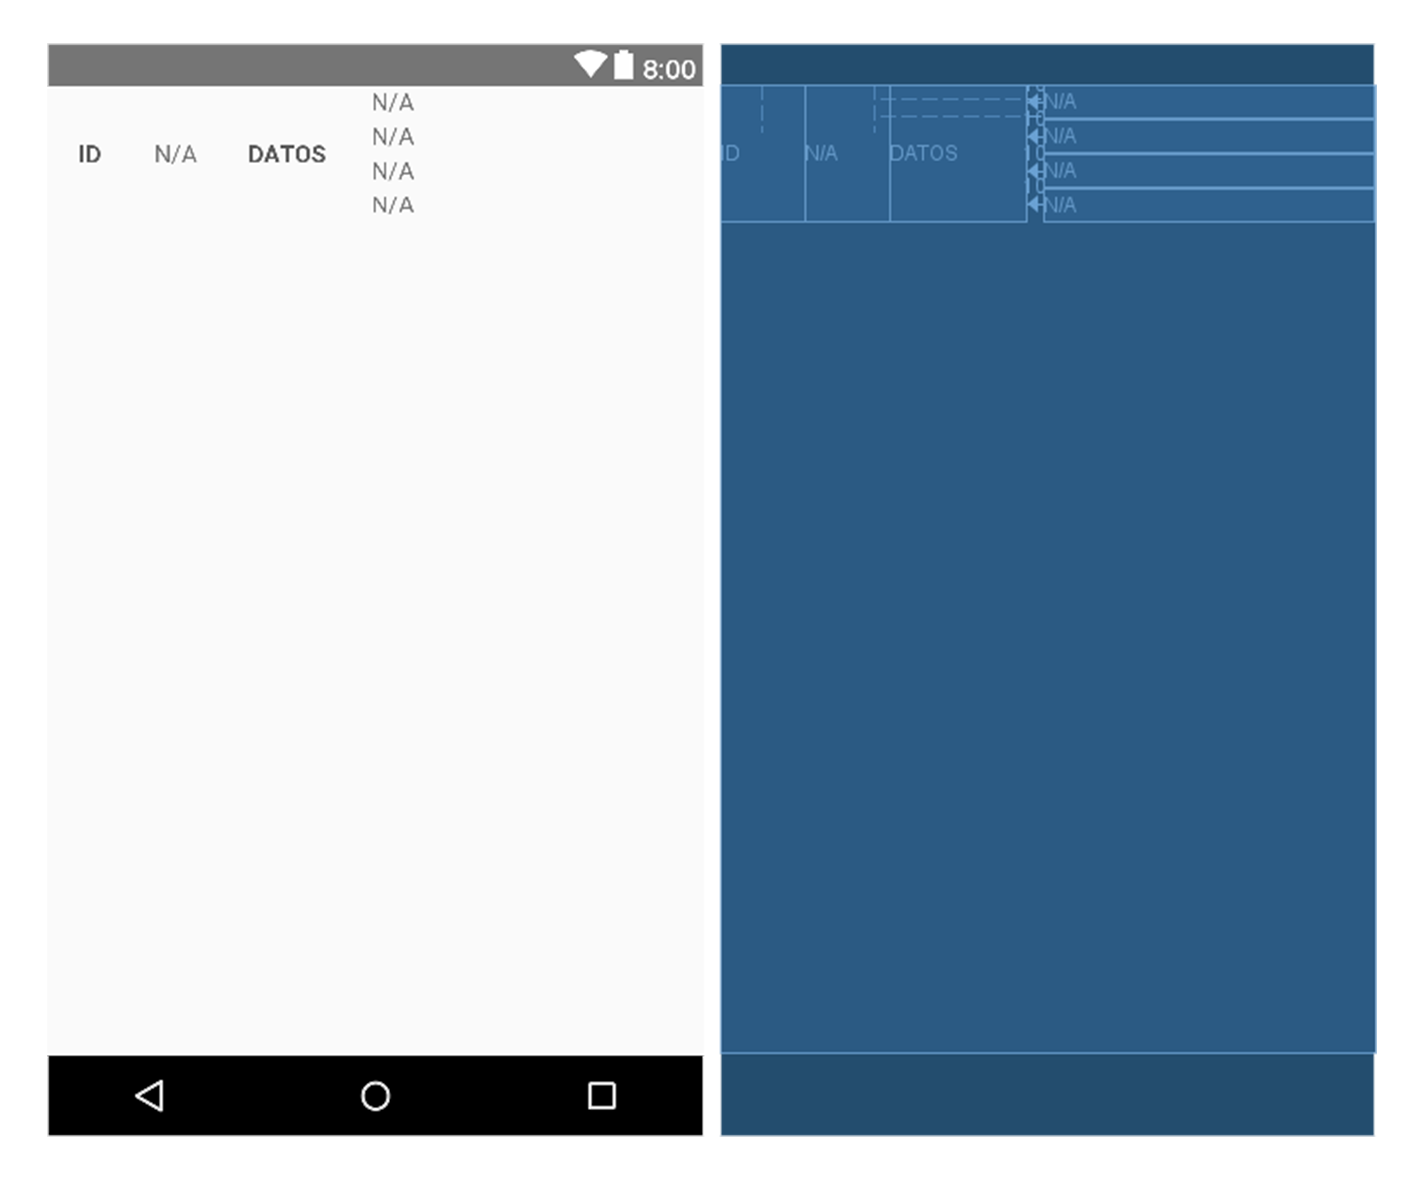
\includegraphics[width=0.5\linewidth]{interfaz4.png}
	\caption{Diseño de interfaz para "ListView" del fragmento recientes y registros}
\end{figure}

\par \noindent
El objetivo de este fragmento es el de mostrar las mediciones realizadas recientemente. Específicamente las ultimas 10 mediciones realizadas en nuestra aplicación. Mas adelante entraremos en detalle a lo que pasa cuando seleccionamos una de las mediciones mostradas en el "ListView". No obstante primero debemos saber cómo ingresamos datos al fragmento recientes. 

\subsubsection{Fragmento Añadir}

\begin{figure}[H]
	\centering
	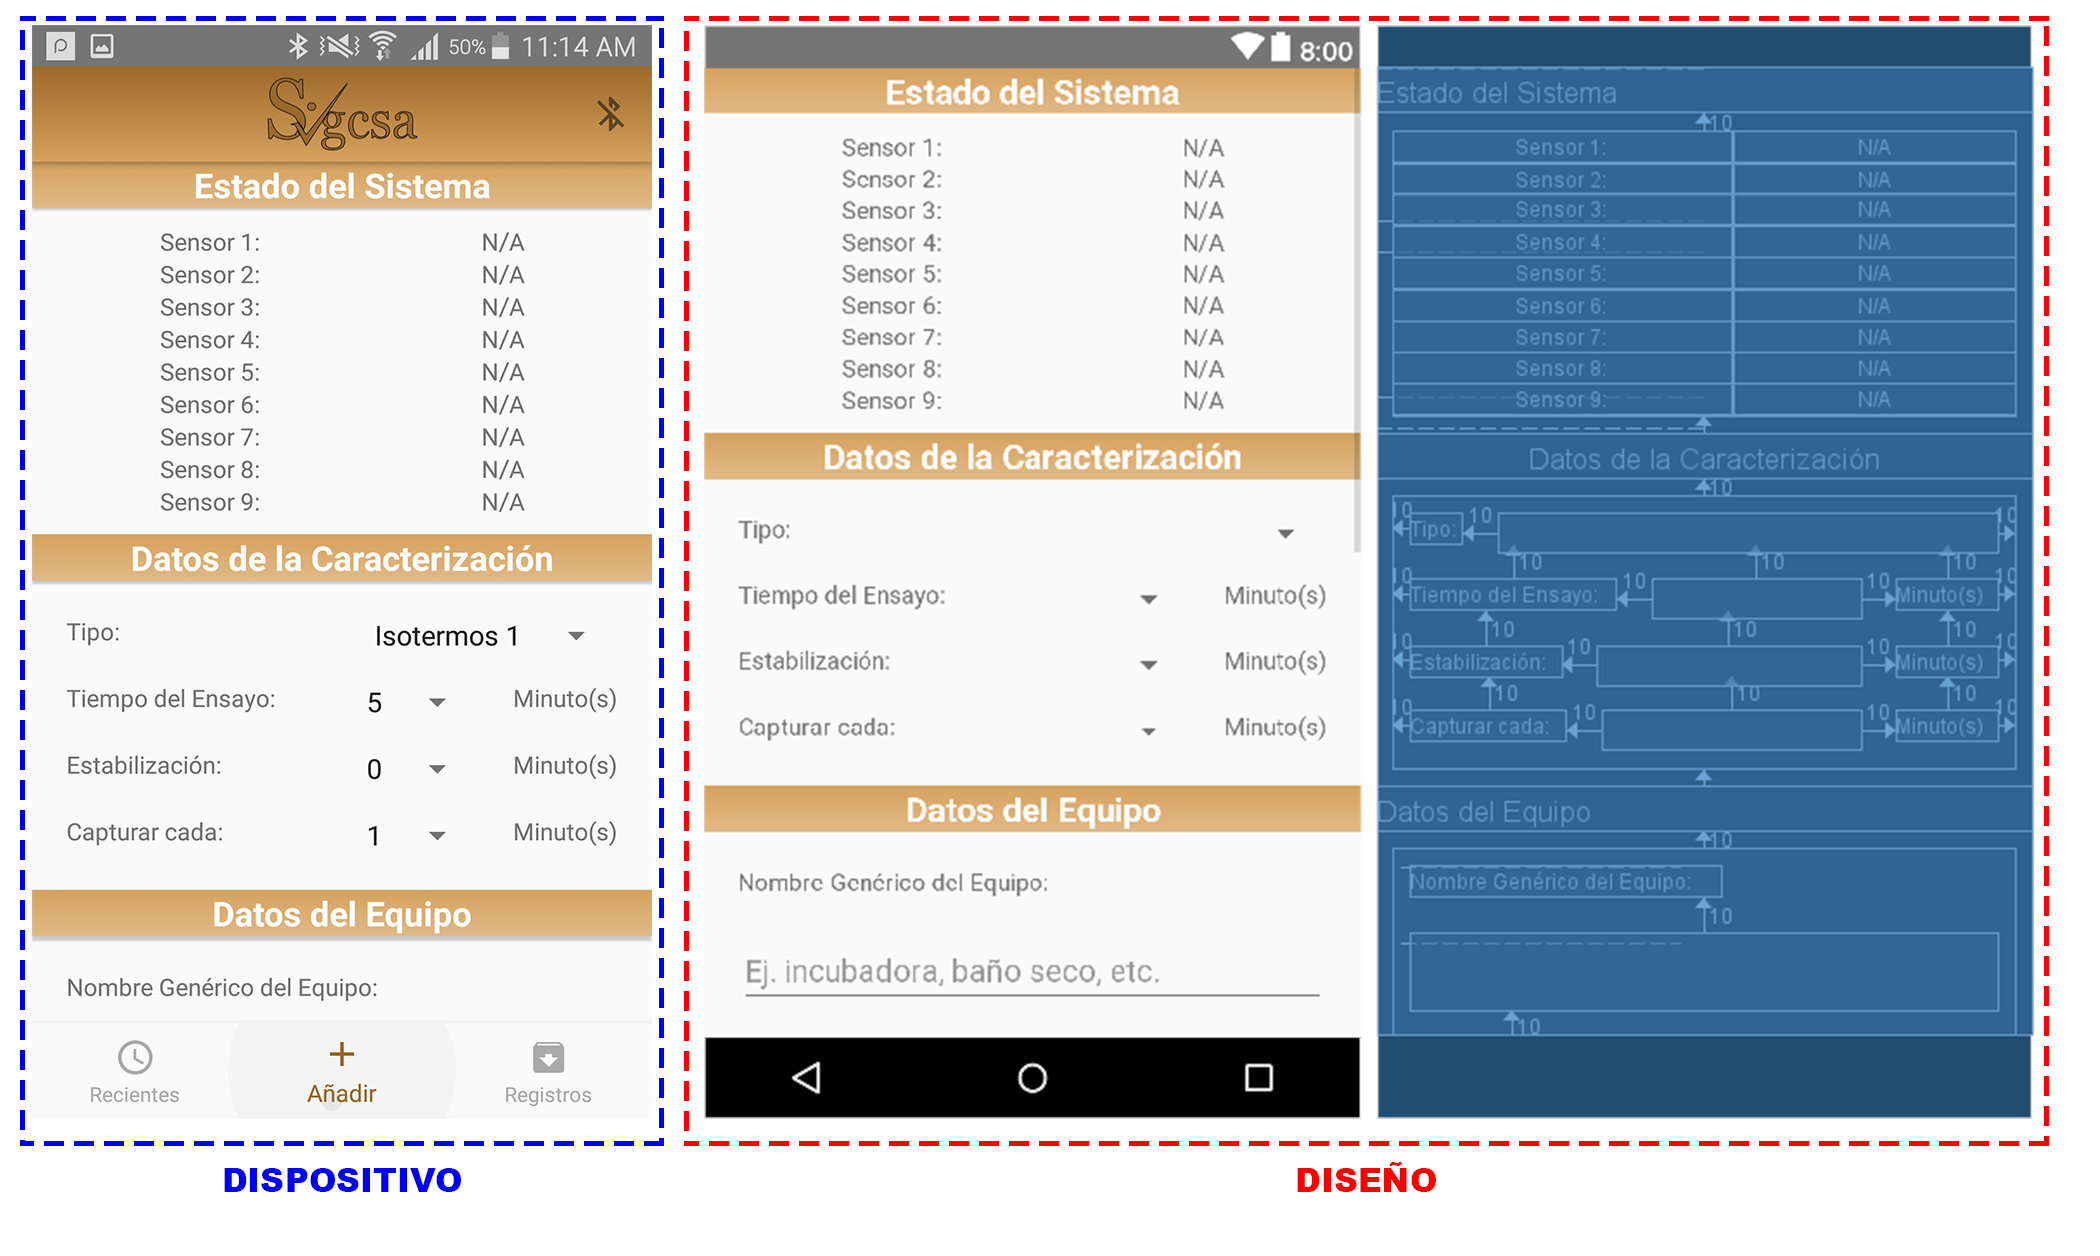
\includegraphics[width=\linewidth]{interfaz5.png}
	\caption{Interfaz del Fragmento Añadir en la aplicación y durante el diseño, parte 1}
\end{figure}

\par 
Fácilmente el fragmento añadir es la interfaz más compleja de este proyecto. El "Layout" utilizado para esta interfaz es un "ScrollView" el cual básicamente es un contenedor con características de desplazamiento vertical. El "ScrollView" es utilizado debido a que todos los elementos de la interfaz no caben en una pantalla promedio de un smartphone. Dentro del "ScrollView" encontramos un "Layout" específicamente un "RelativeLayout" el cual permite un manejo eficiente de los elementos que conforman la interfaz del usuario. 

\par \noindent
El fragmento añadir se divide en 3 secciones. Al inicio el "Estado del Sistema", seguido de “Datos de la Caracterización" y "Datos del Equipo". Estas secciones son dividas por un simple texto con fondo; con el objetivo de mantener la aplicación fluida al usuario.

\begin{figure}[H]
	\centering
	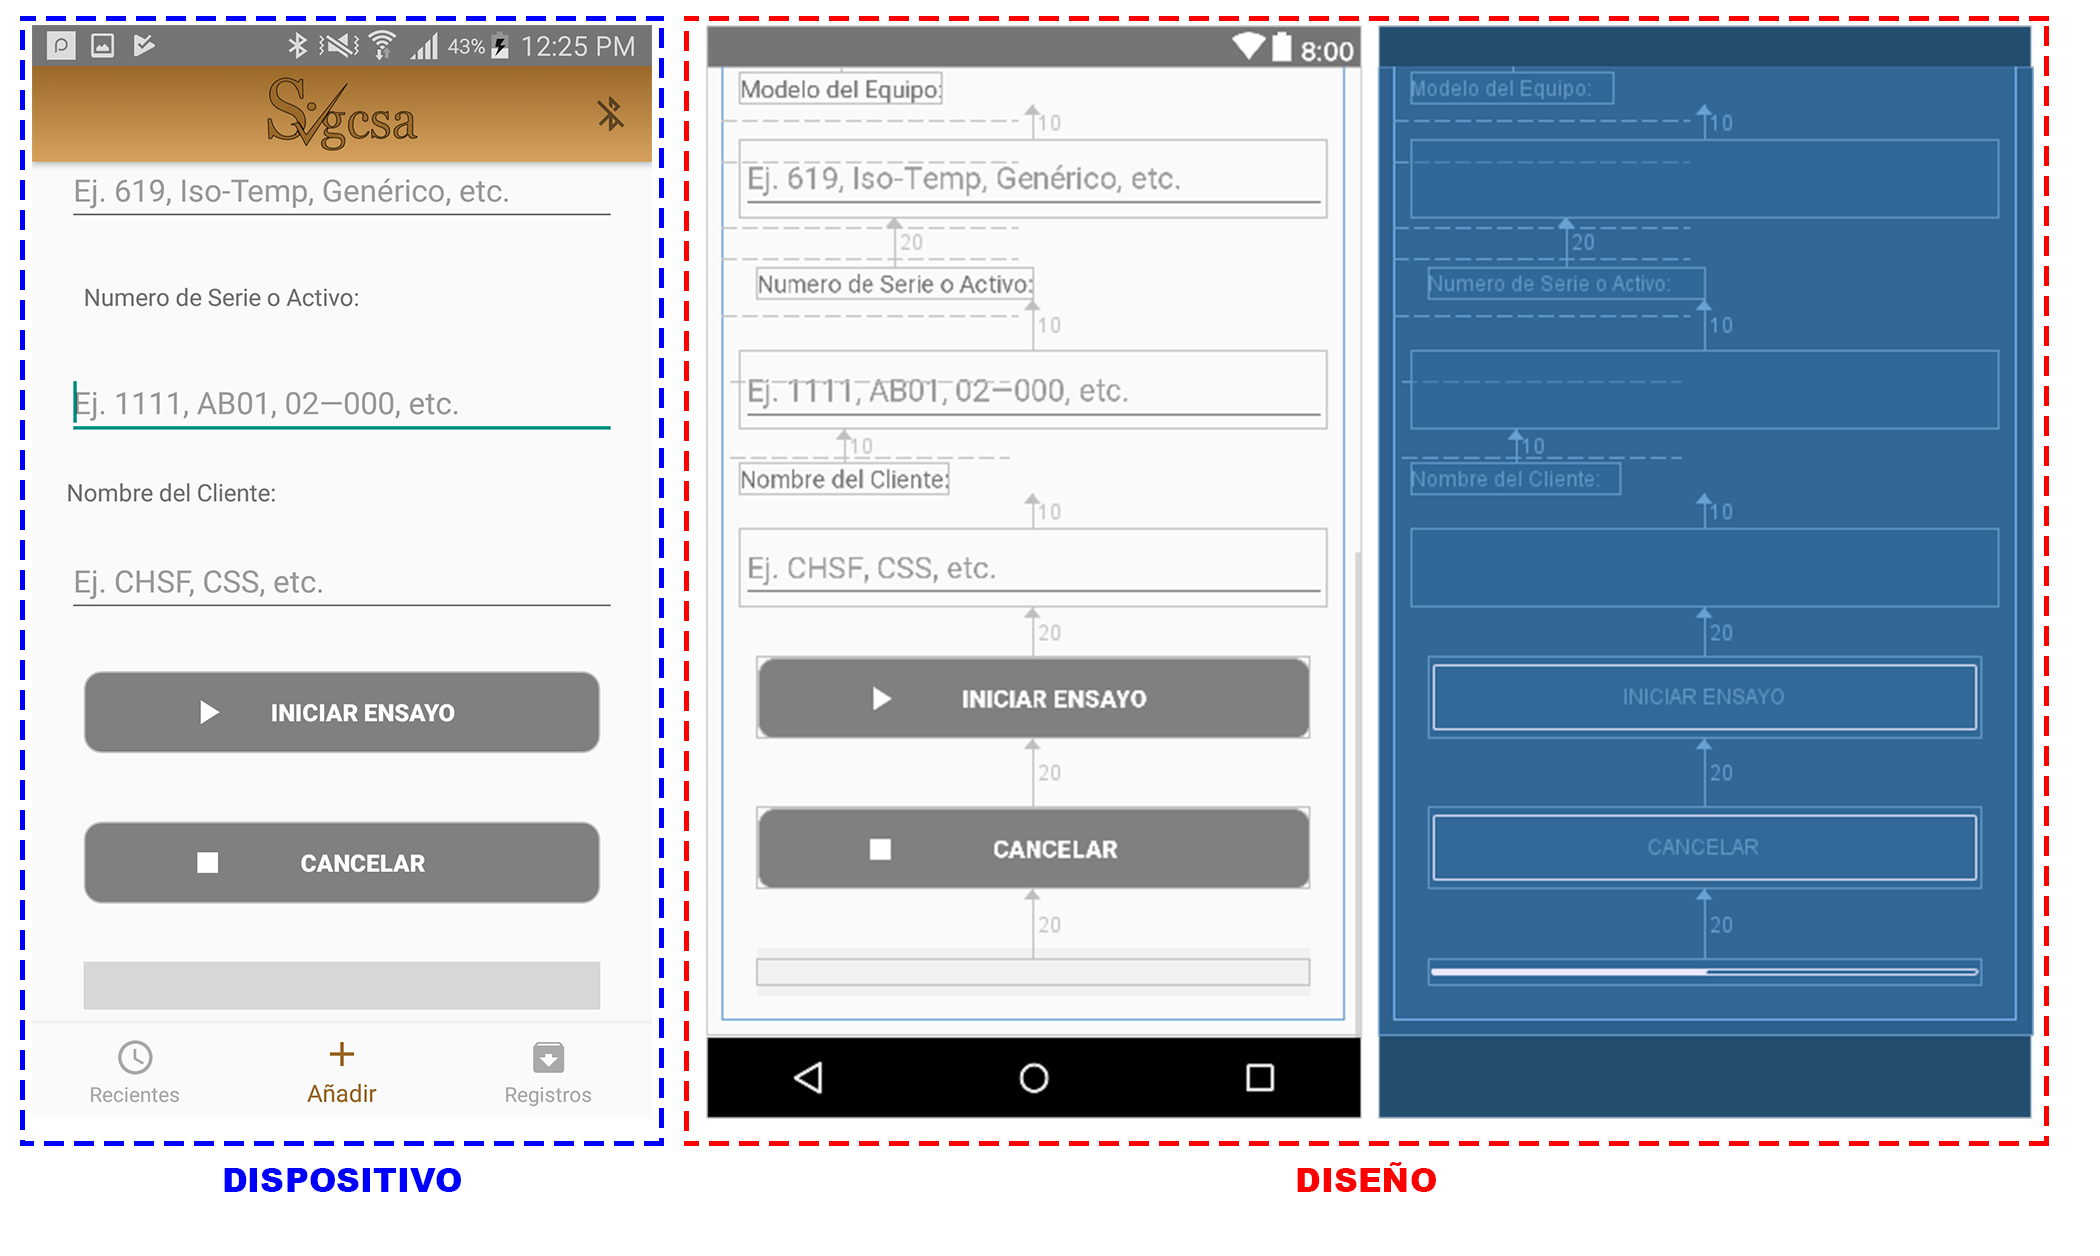
\includegraphics[width=\linewidth]{interfaz6.png}
	\caption{Interfaz del Fragmento Añadir en la aplicación y durante el diseño, parte 2}
\end{figure}

\par \noindent
La sección "Estado del Sistema" contiene los textos que visualizaran las temperaturas de los prototipos; ver imagen 3.13, una vez sea establecida la comunicación por bluetooth. A la izquierda es una guía del número de sonda o prototipo y a la derecha se encuentra el texto "N/A"; sin embargo, este valor cambiará a la temperatura actual obtenida por su respectivo prototipo y en caso tal de no recibir una lectura se mantendrá en el texto "N/A".

\par \noindent
La sección "Datos de la Caracterización" contiene los parámetros que definirá el usuario para determinar las características de la medición o ensayo. En la imagen 3.13 podemos observar que esta sección consta de 4 casillas donde el usuario puede elegir opciones predeterminas.

\par \noindent
En las opciones de tipo hay 3 opciones: Isotermos 1, Isotermos 2 y Calibración con Patrón. Según el capítulo 3 donde se analizaron los procesos a automatizar podemos notar que los medios Isotermos 1 necesitan de 9 termómetros; mientras que, Isotermos 2 de 4 termómetros. Al saber esto debemos tener una interfaz dinámica; la cual dependiendo del tipo de ensayo que se seleccione muestre únicamente la cantidad de prototipos que necesitaremos. 

\begin{figure}[H]
	\centering
	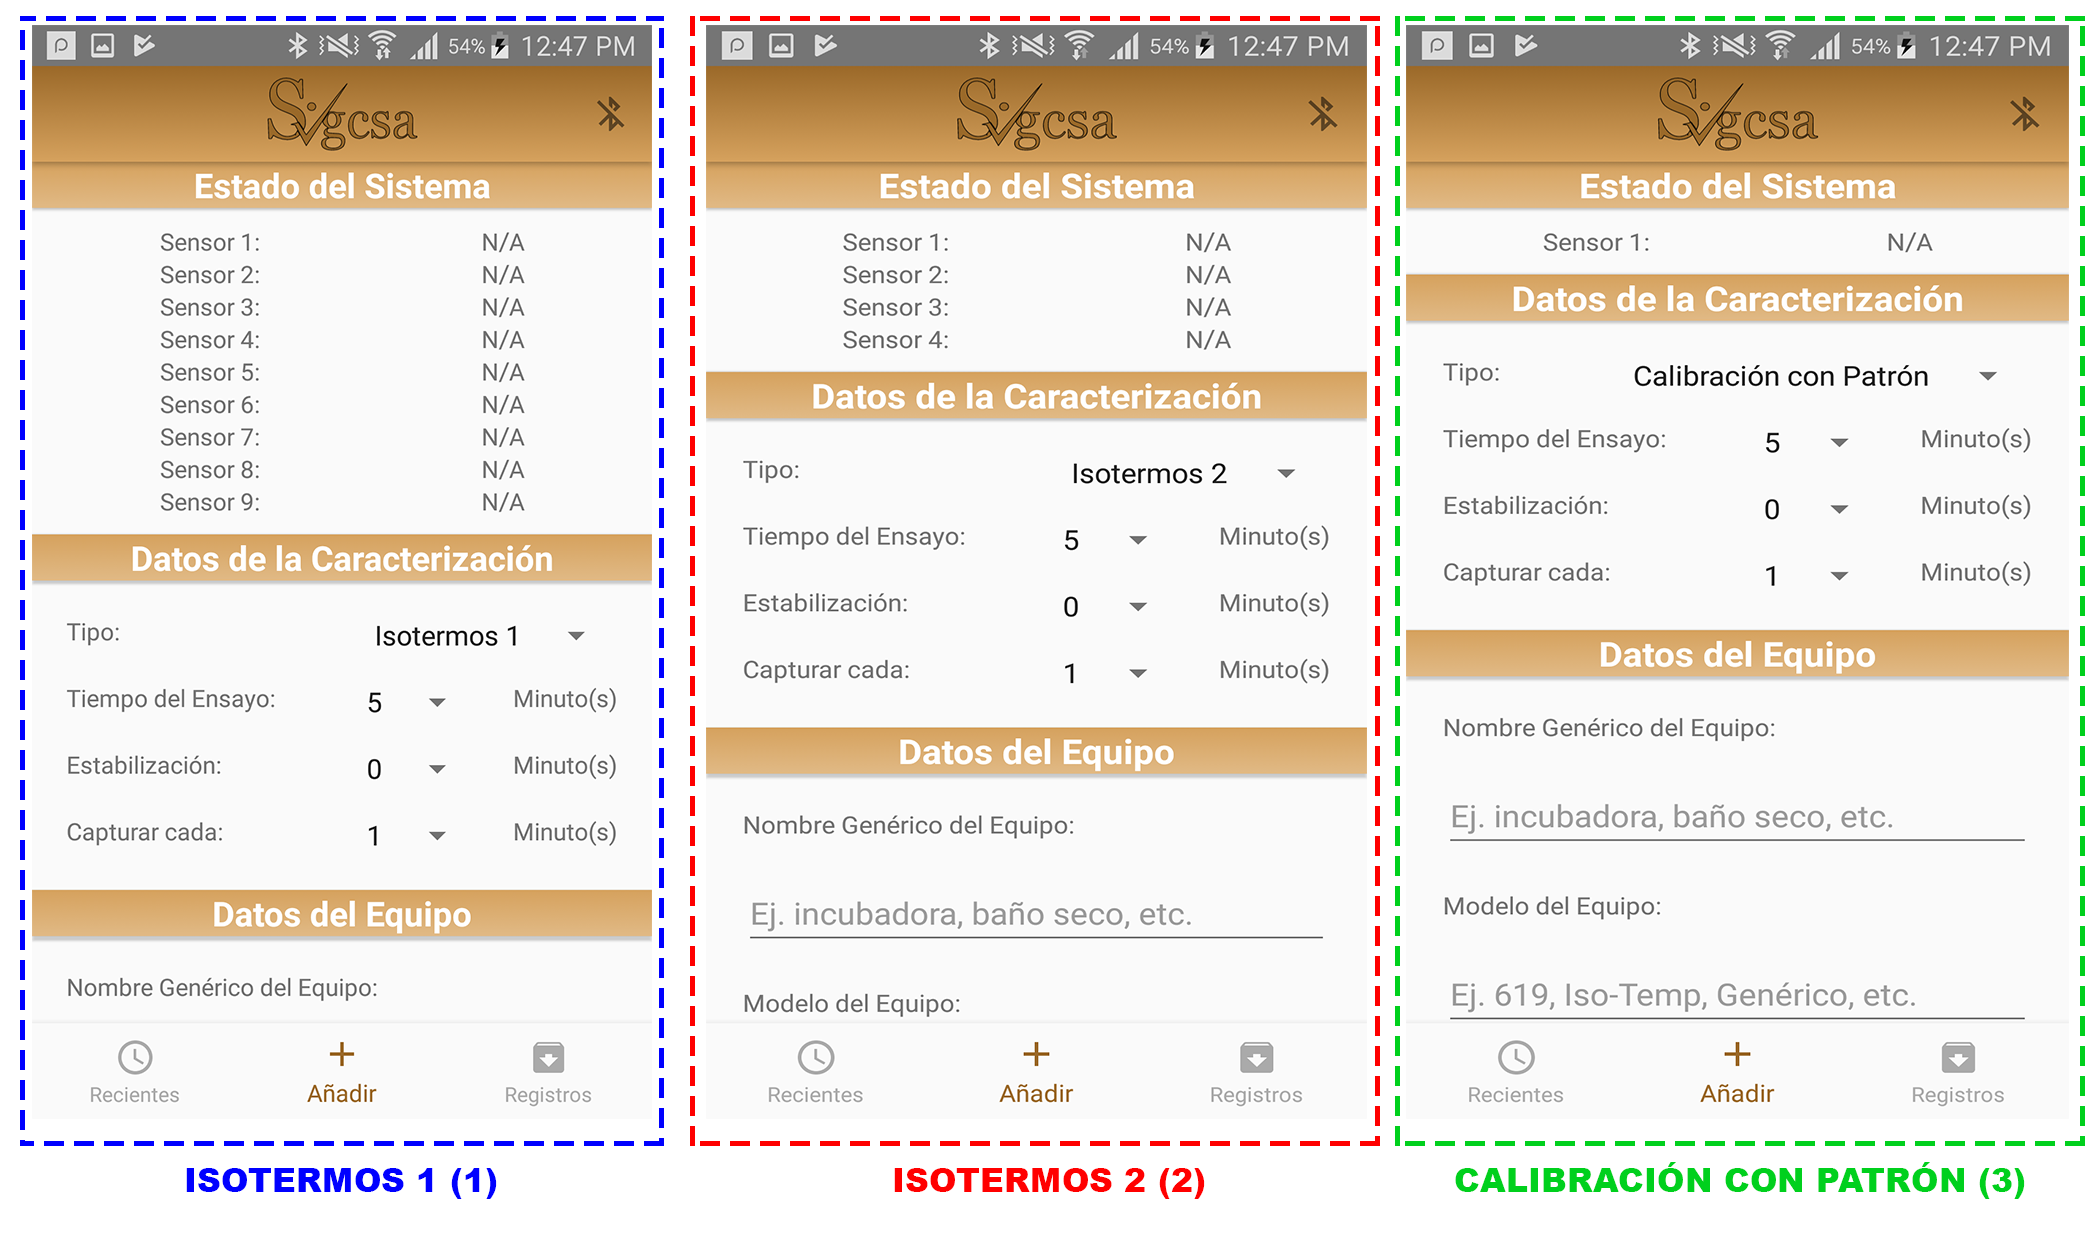
\includegraphics[width=\linewidth]{interfaz7.png}
	\caption{Dependiendo de la opción seleccionada, se ajustan los textos en la sección de "Estado del Sistema"}
\end{figure}

\par \noindent
Entre los otros parámetros de la sección "Datos de la Caracterización" se encuentran las casillas para "tiempo del ensayo" el cual determinará por cuanto tiempo se tomará las medidas de temperatura donde el mínimo son 5 minutos y el máximo es de 60 minutos o una hora. "Estabilización" es el tiempo previo que seleccionara el usuario final; en muchas ocasiones personal de campo esperan que la temperatura en un medio isotermo se estabilice antes de proceder a capturar las medidas. Por último "Capturar cada" se explica por sí misma, es el intervalo de tiempo en que se tomaran las medidas de temperatura.

\par \noindent
Como hemos mencionado esta interfaz contiene más componentes que las demás; por lo que, no todos los componentes de la interfaz pueden ser apreciados en una pantalla de un smartphone promedio. Se debe deslizar el fragmento para poder observar los componentes faltantes. Una vez realizado esto la interfaz quedara como la imagen 3.14. 

\par \noindent
La última sección "Datos del Equipo" cuenta con campos para ingresar información del equipo a realizar el ensayo de caracterización. Datos como nombre, modelo, serie y cliente. Adicional contamos con dos botones, uno para iniciar el servicio para el registro de mediciones y otro para cancelar dicho servicio. Por último hay un "progressbar" el cual se irá completando a medida que vaya avanzando el ensayo.

\subsubsection{Fragmento Registros}

\begin{figure}[H]
	\centering
	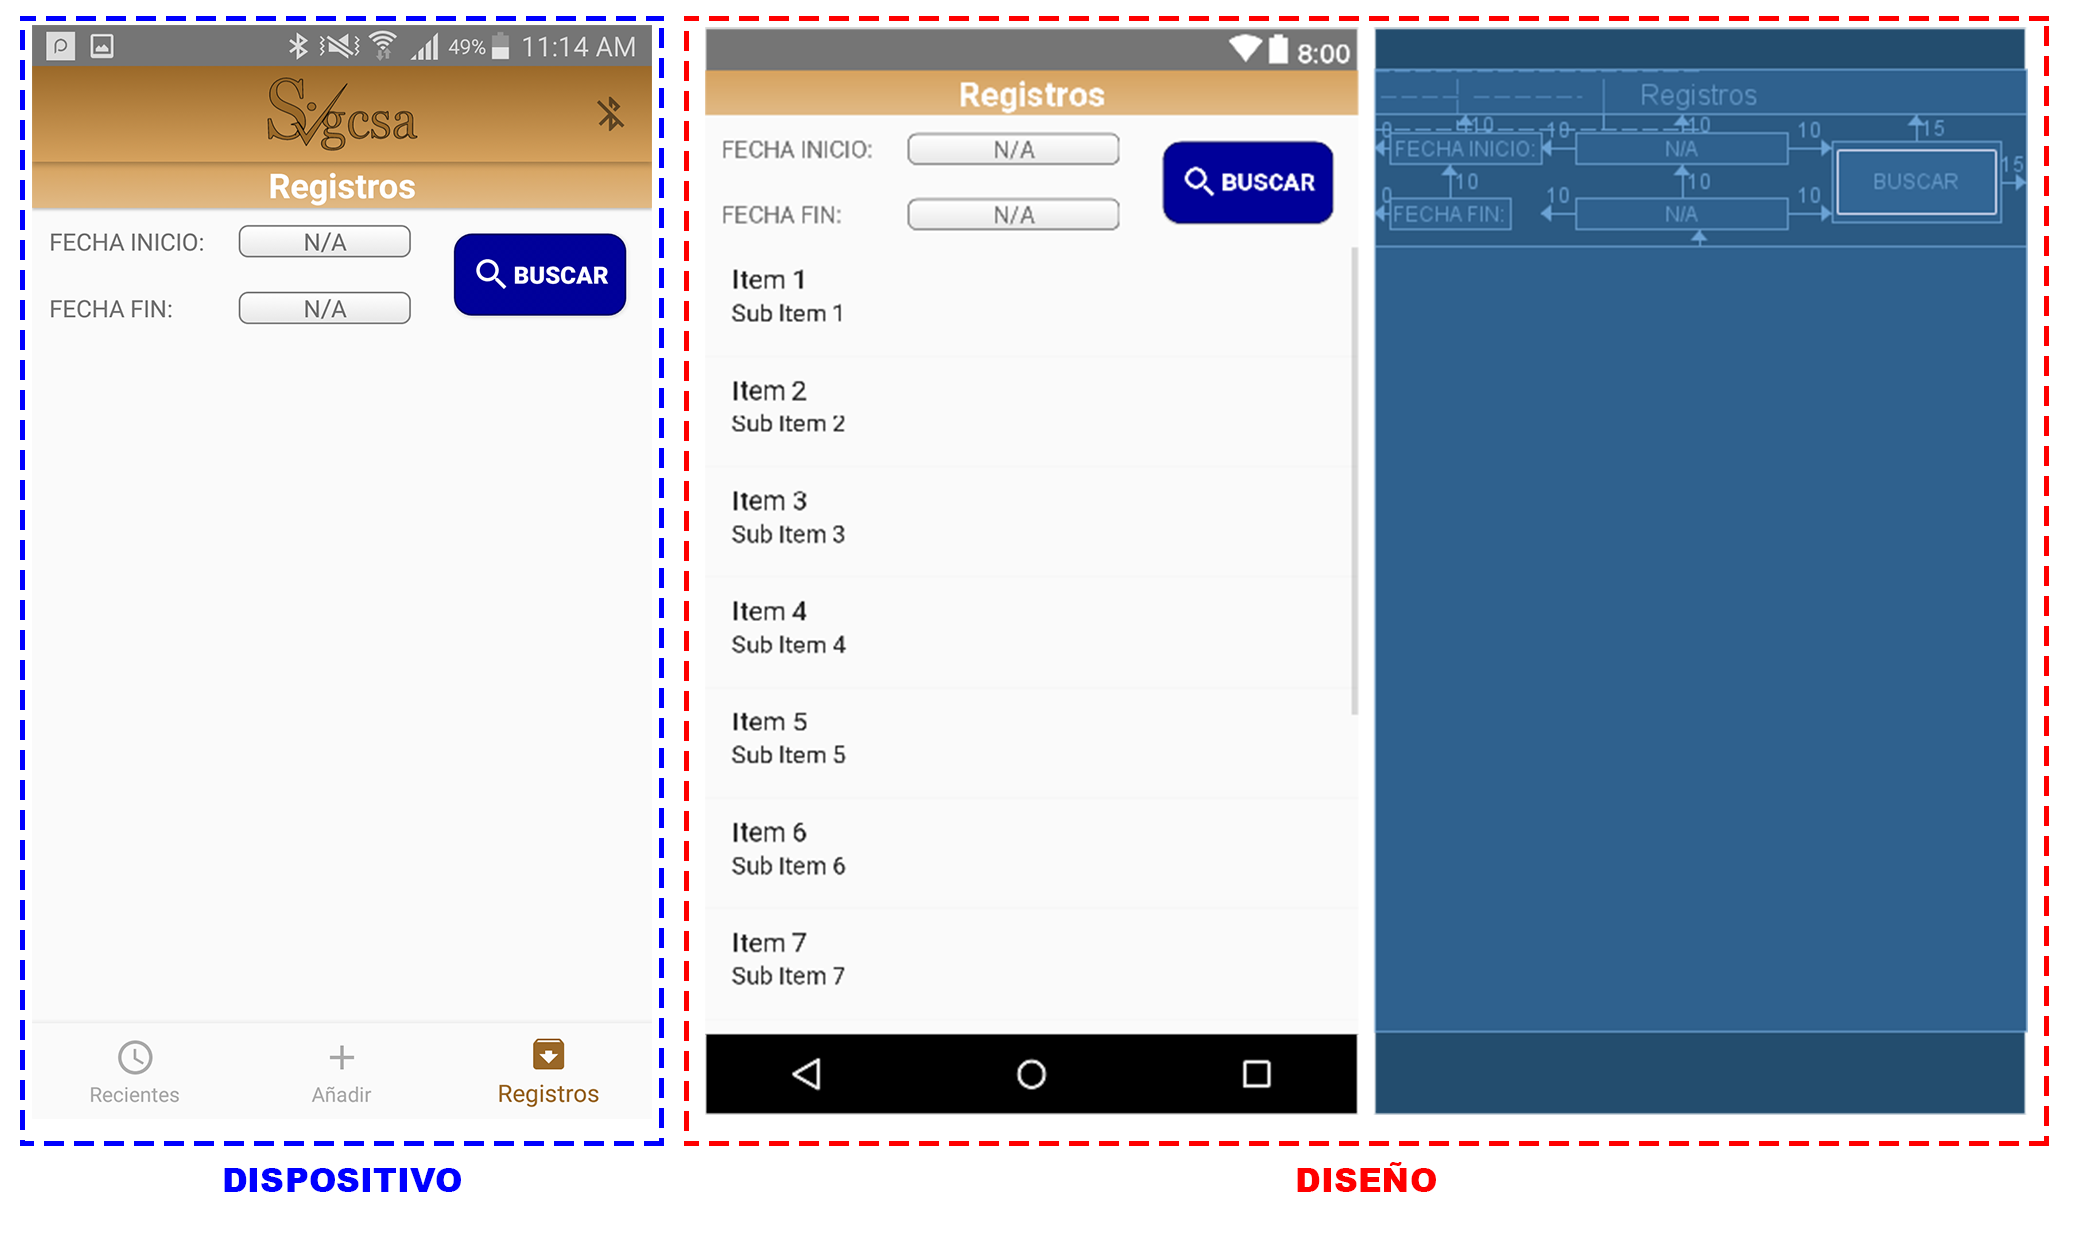
\includegraphics[width=\linewidth]{interfaz8.png}
	\caption{Interfaz y diseño del fragmento registros}
\end{figure}

\begin{figure}[H]
	\centering
	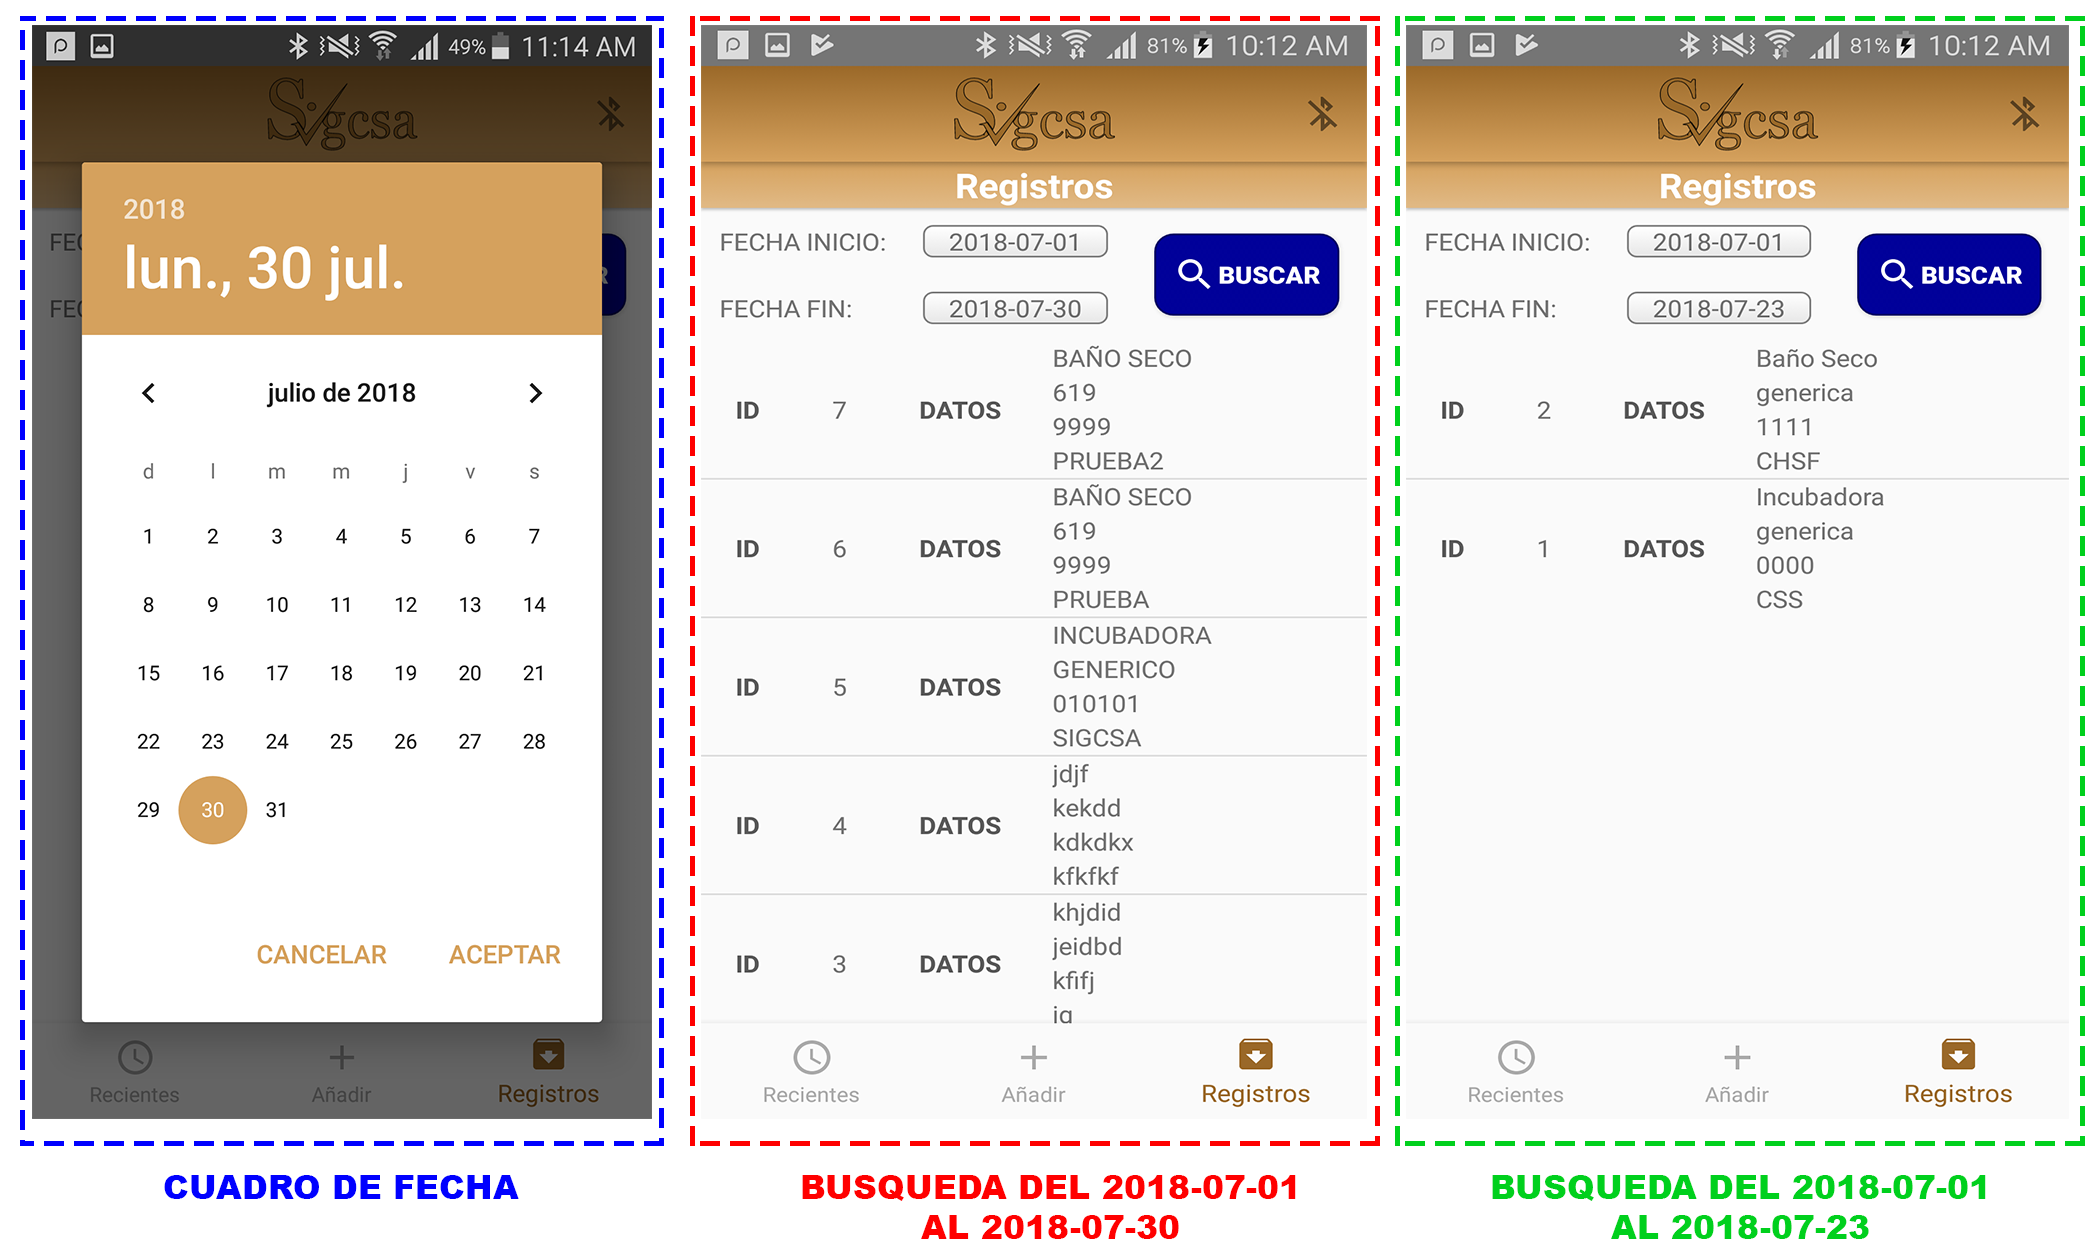
\includegraphics[width=\linewidth]{interfaz9.png}
	\caption{Cuadro de selección de fechas y resultados del fragmento registros dependiendo de la fecha}
\end{figure}

\par
El fragmento registros básicamente es una extensión del fragmento recientes, la única diferencia es que se puede definir las fechas de las mediciones (ensayos) que hemos realizado en nuestro smartphone. 

\par \noindent
Cuenta con textos que indican los botones para seleccionar fecha de inicio y fecha fin, al seleccionar uno de los botones se abre un cuadro con una interfaz amigable, ver imagen 3.17, para seleccionar la fecha deseada. Un botón de buscar el cual buscara las mediciones en la base de datos utilizando como parámetros las fechas seleccionadas. De encontrar resultados los despliega en un "ListView" del fragmento en cuestión. El comportamiento del "ListView" del fragmento registros es igual al del fragmento recientes.

\par \noindent
Estos tres fragmentos componen la actividad principal. Ya sabemos que es la primera que visualiza el usuario después de la animación inicial. Sabemos también que es donde se consulta la información de los ensayos realizados, estipulamos los parámetros de un ensayo, lo iniciamos o cancelamos y tenemos conocimiento en tiempo real de las temperaturas de los prototipos. Pero aún no sabemos dónde establecemos comunicación con nuestro prototipo. 

\subsubsection{Actividad Bluetooth}

\par 
La actividad bluetooth es la encargada de visualizar los equipos bluetooth disponibles. Establece comunicación con nuestro prototipo; ya que, es la encargada de llamar al servicio bluetooth de nuestra aplicación; la cual retroalimenta la actividad principal.

\par \noindent
En las imágenes 3.13, 3.14, 3.15, 3.16 y 3.17 podemos percatar en la esquina superior derecha de nuestra aplicación un pequeño icono de color gris con un símbolo de bluetooth. Si seleccionamos este icono llamamos a la actividad bluetooth. En ella podemos visualizar los dispositivos bluetooth disponibles. Está compuesta por un "toolbar" que con el texto "Conexiones Bluetooth" y botón para regresar a la actividad principal. Un texto con fondo que indica los dispositivos, un "ListView" en el cual se desplegaran los dispositivos disponibles. Por último un botón para actualizar el "ListView" en caso tal de querer establecer una conexión con nuevos dispositivos.

\begin{figure}[H]
	\centering
	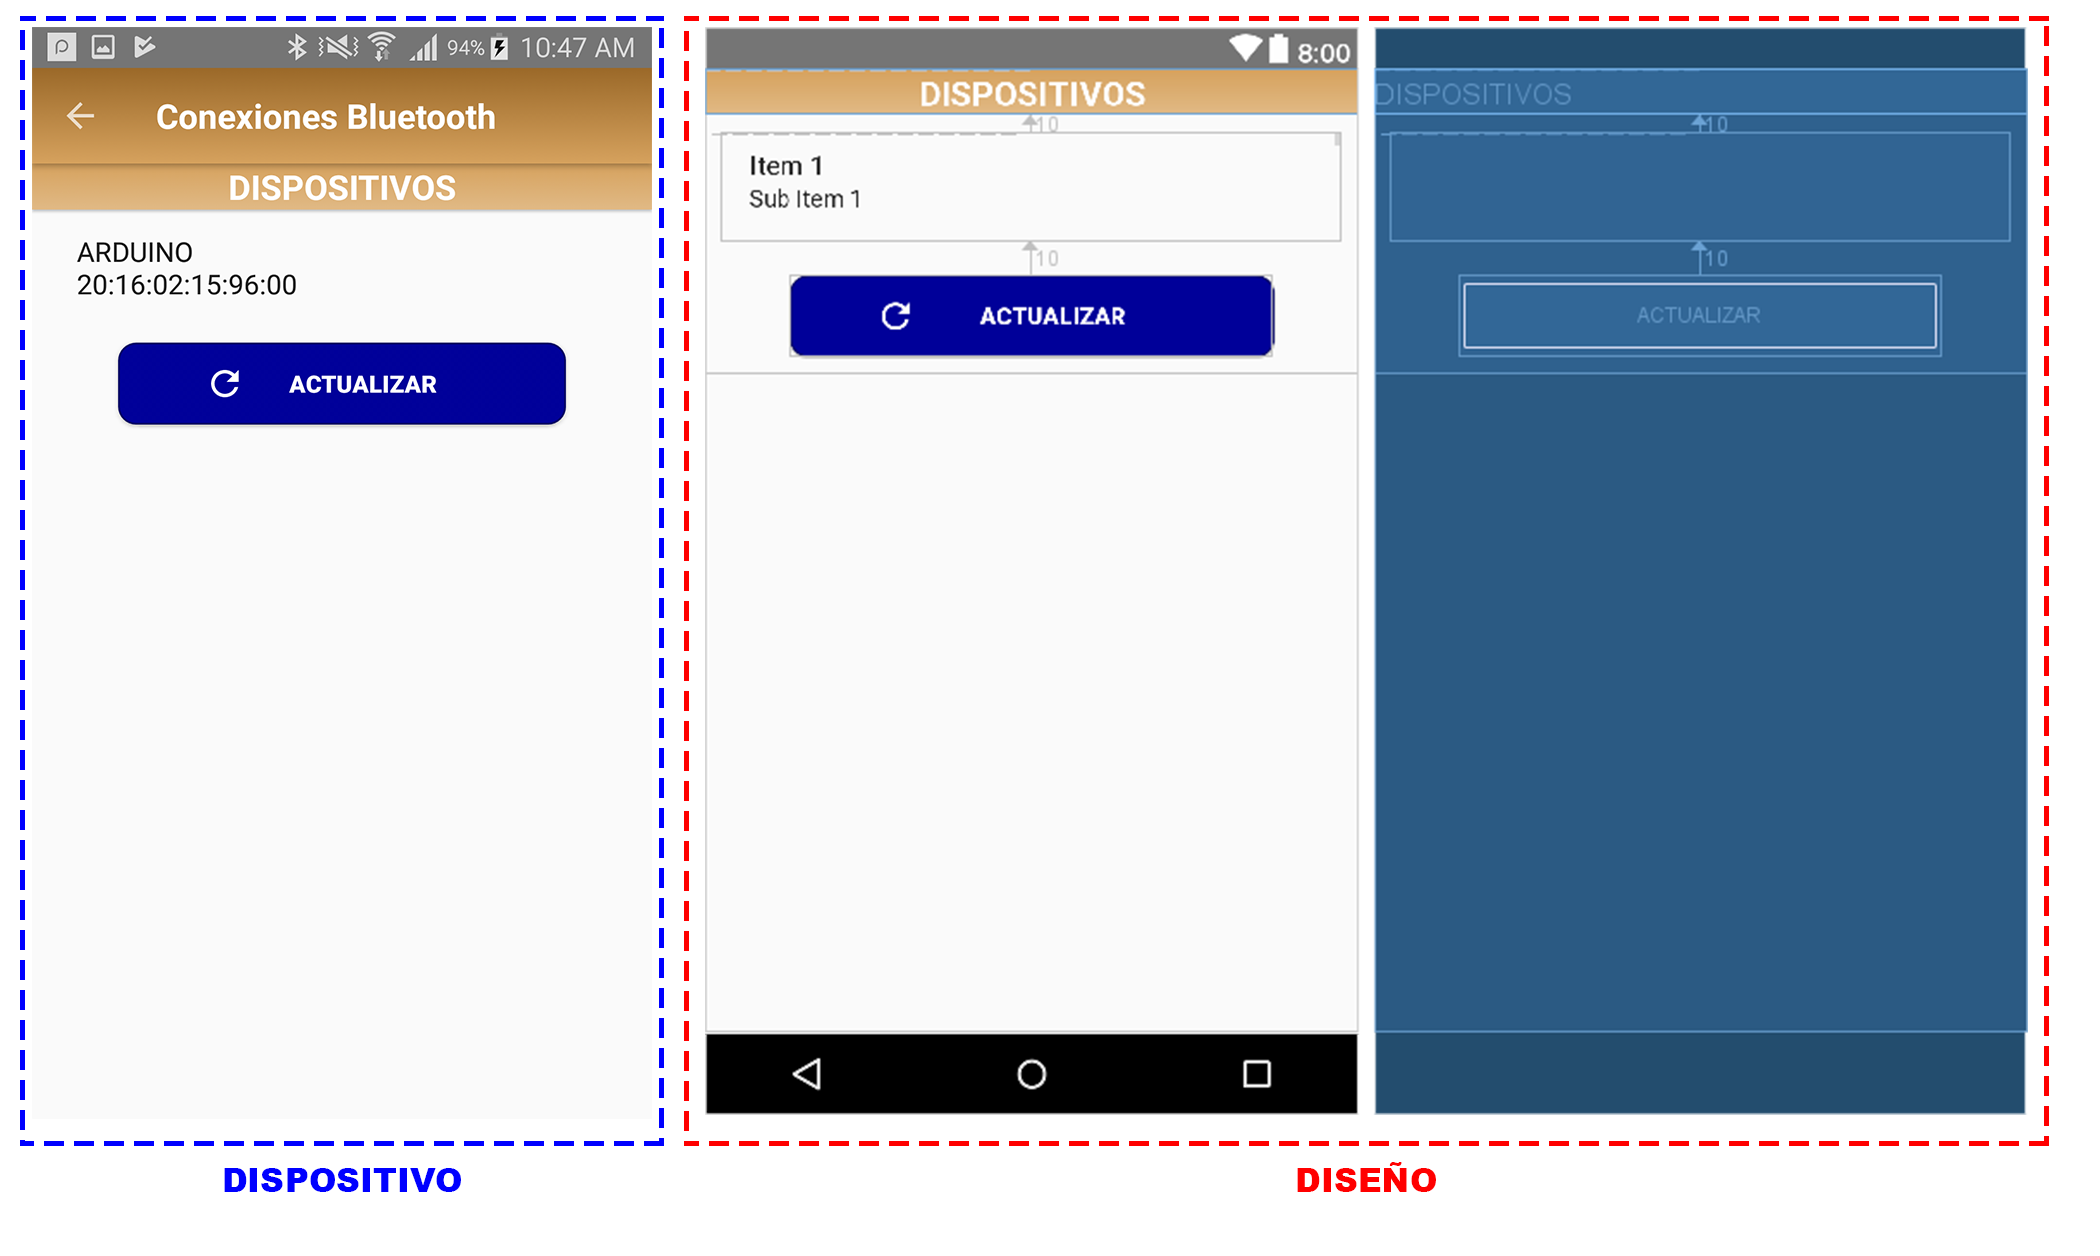
\includegraphics[width=\linewidth]{interfaz10.png}
	\caption{Interfaz y diseño de la actividad bluetooth}
\end{figure}

\par \noindent
La última tarea o función de que el usuario puede realizar en nuestra aplicación es el de consultar la información capturada. La actividad detalle es la encargada de demostrar la información capturada en los ensayos y las mediciones de los prototipos. Anteriormente en la sección de fragmento recientes y registros habíamos mencionado que el componente "ListView" tiene muchas características y que una de ellas era la de simular un botón por cada renglón de información desplegada al usuario. La actividad detalle es ejecutada al seleccionar una de la opción de los "ListView".

\subsubsection{Actividad Detalle}

\par 
En las imágenes 3.11 y 3.17 podemos observar los "ListView" donde se despliegan información de los ensayos realizados en la aplicación. Cada opción de ambas listas cuenta con información del ensayo que se encuentra en la base de datos de la aplicación. Al seleccionar una de las opciones se desplegará la actividad detalle. 

\par \noindent
En la Imagen 3.19 observamos que en la información y componentes de la interfaz se encuentran distribuida de manera similar al del fragmento añadir.

\begin{figure}[H]
	\centering
	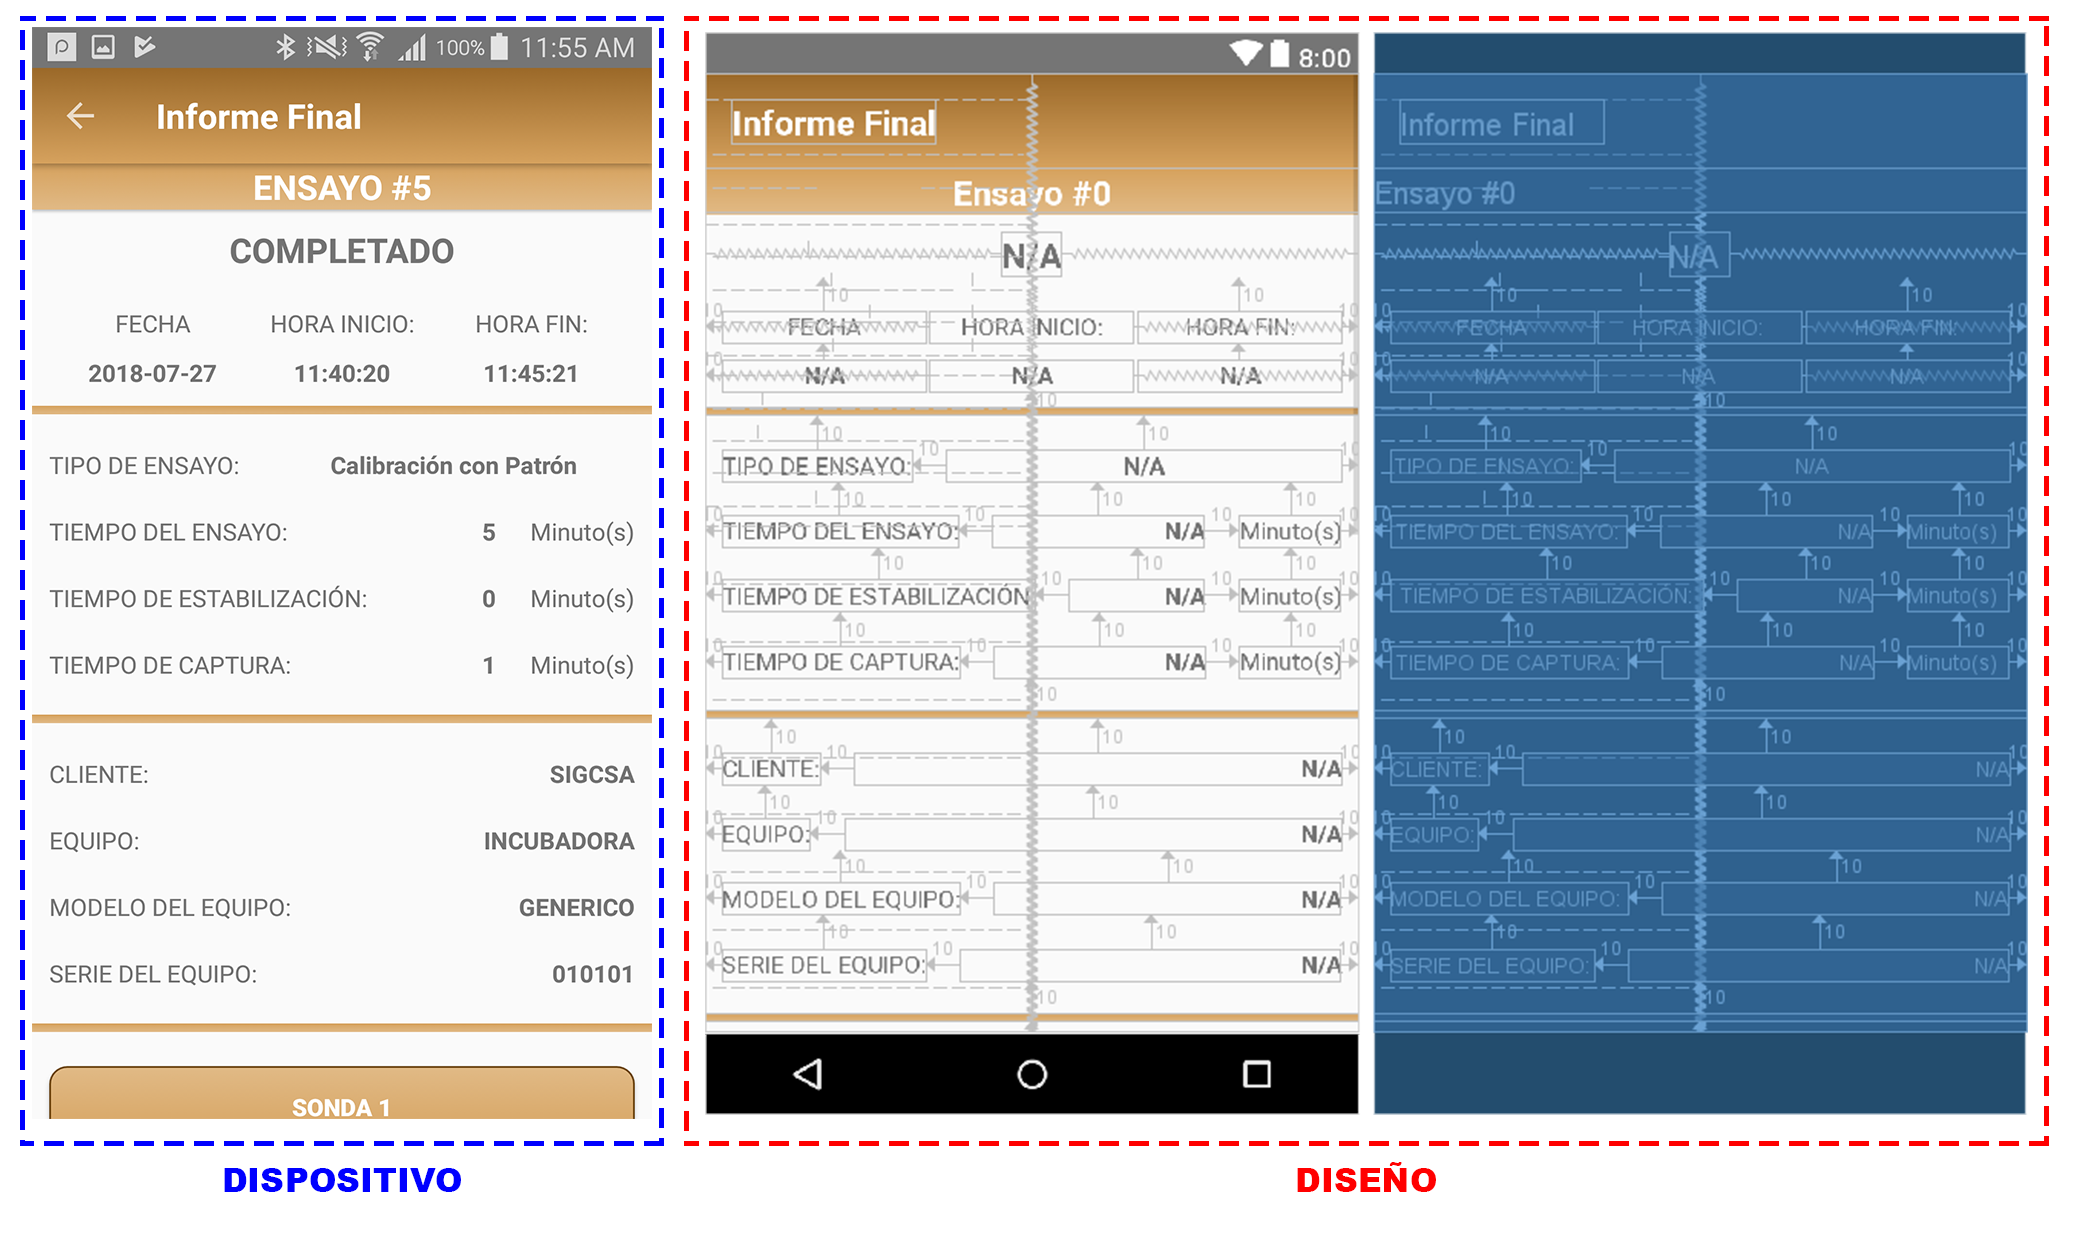
\includegraphics[width=\linewidth]{interfaz11.png}
	\caption{Interfaz y diseño de la actividad detalle}
\end{figure}

\par \noindent
Al inicio de la interfaz de esta actividad se encuentra el "toolbar" o barra de navegación con el texto "Informe Final" y un botón para regresar a la actividad principal. Seguido un texto con un fondo del color de la aplicación con el texto "Ensayo" junto con su respectivo ID en la base de datos. En la primera sección se indica al usuario si el ensayo fue "COMPLETADO" en caso tal que no haber ningún problema durante la captura de la información y en caso contrario que el usuario haya presionado el botón cancelar el texto será "CANCELADO". Luego datos esenciales como la fecha de ejecución del ensayo, hora de inicio del ensayo y hora de finalización del ensayo.

\par \noindent
Luego sigue información de los parámetros seleccionados y escritos por el usuario para el ensayo. Por último se encuentra un botón con el texto "Sonda 1". La cantidad botones dependerá del tipo de ensayo que se ha realizado. De la misma manera como es dinámico el texto del "Estado del Sistema" en el fragmento añadir. Estos botones son especiales ya que al presionarlos se inicia la actividad detalle sonda.

\subsubsection{Actividad Detalle Sonda}

\begin{figure}[H]
	\centering
	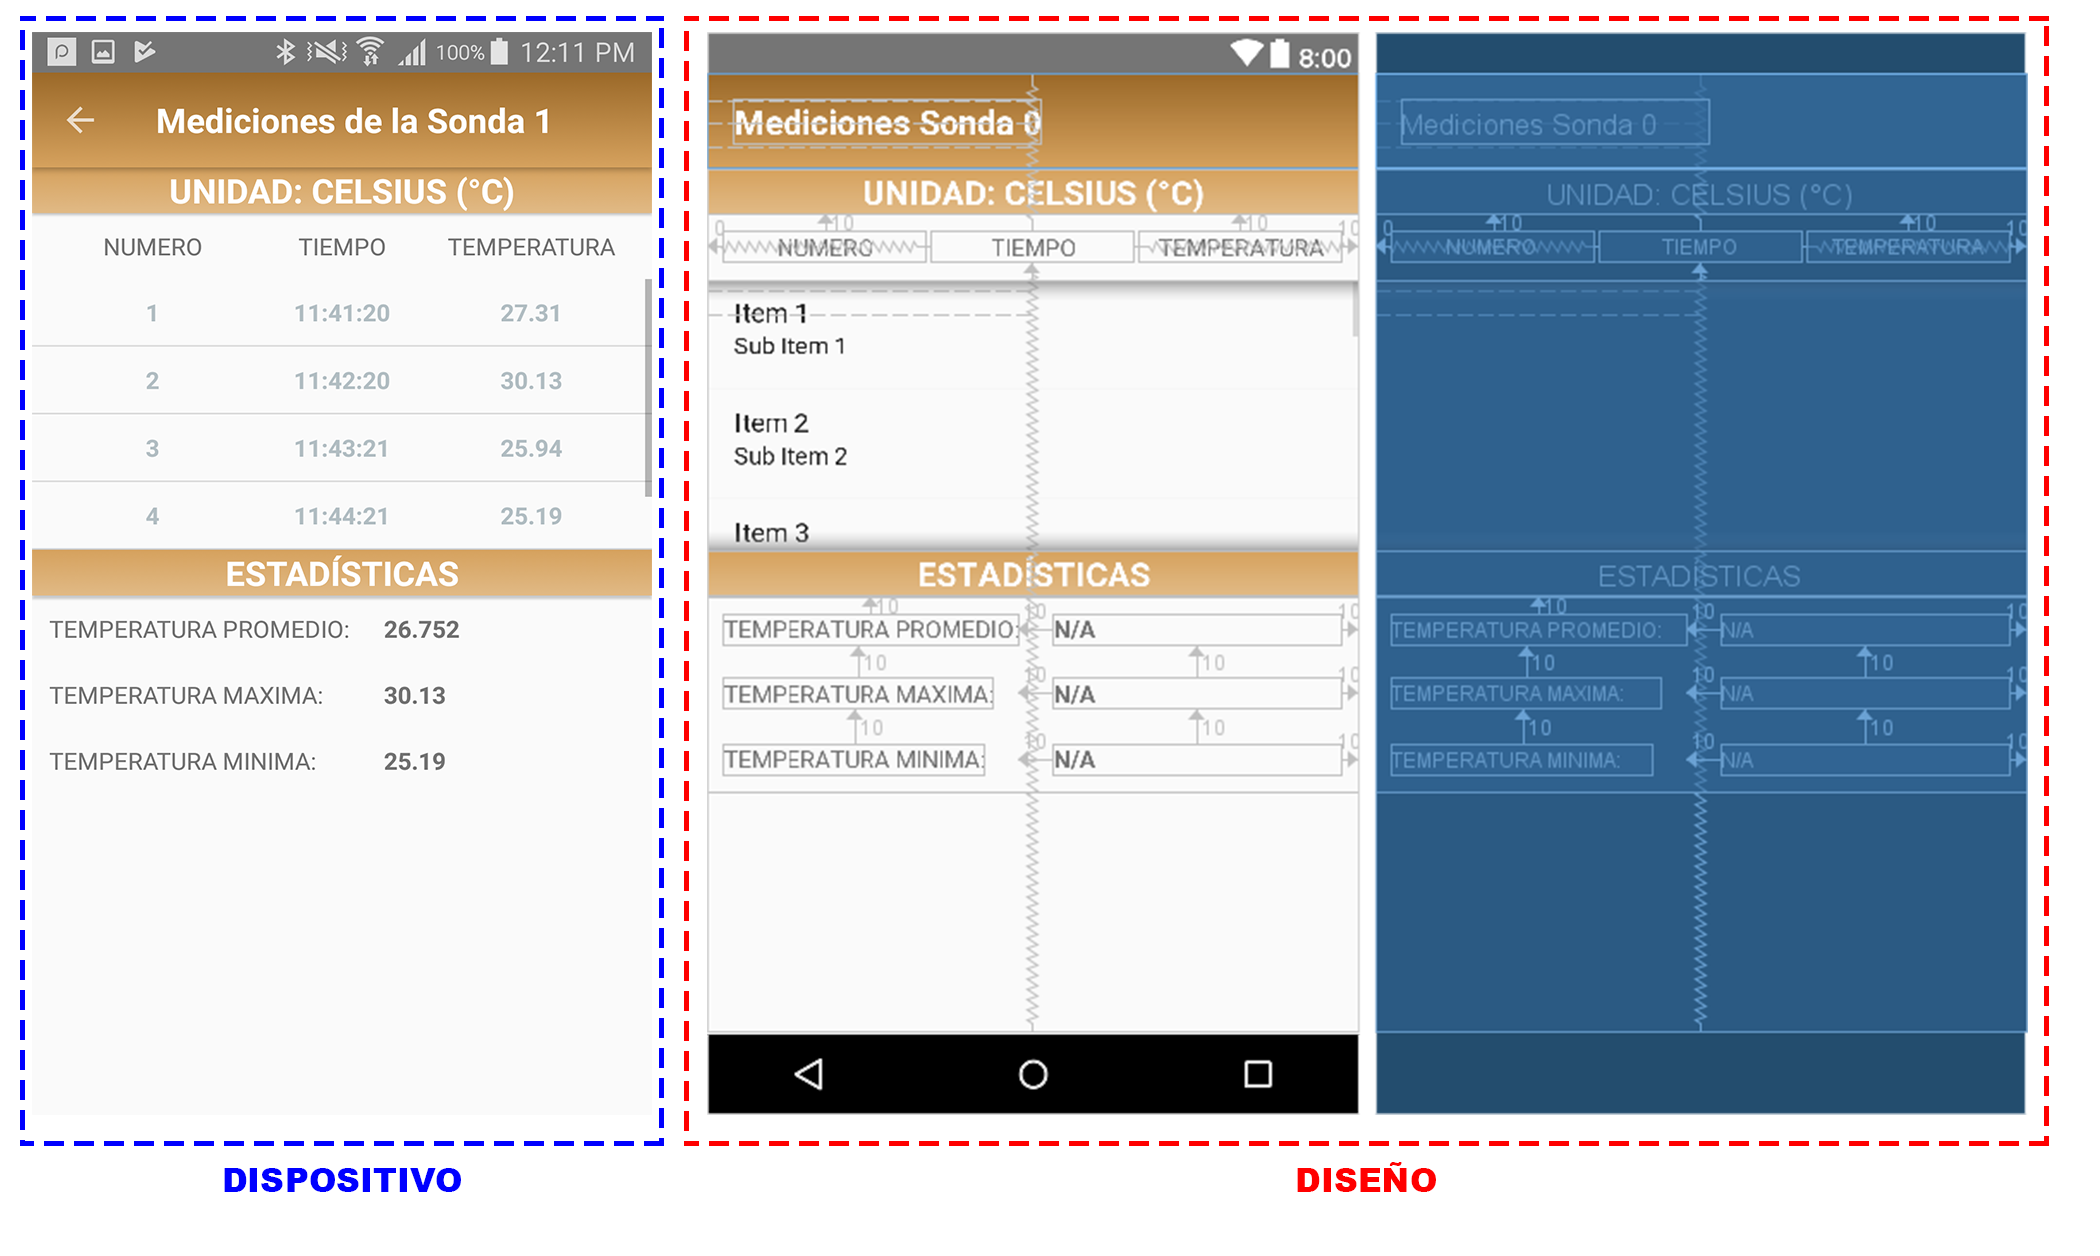
\includegraphics[width=\linewidth]{interfaz12.png}
	\caption{Interfaz y diseño de la actividad detalle}
\end{figure}

\par \noindent
La actividad detalle sonda es donde se muestran las mediciones de temperaturas capturadas por la sonda de un prototipo. Pero ¿Por qué una actividad o una interfaz para cada sonda? recordemos que en Android hay que mantener la aplicación fluida para una buena experiencia del usuario. En el peor de los casos si el usuario selecciona un tipo de caracterización "Isotermos 1" donde se tomará las mediciones de 9 sondas y si se selecciona capturar cada minuto tenemos un total de 60 mediciones por 9 sondas. Esto puede afectar el rendimiento de la aplicación al renderizar esa gran cantidad de texto en menos de 1 segundo.

\par \noindent
Otra de las razones es para mantener mejor organizada la información y una interfaz más amigable. La interfaz de la actividad detalle sonda consta de un "toolbar" con un texto indicando su respectiva sonda y un botón para regresar a la actividad detalle. Seguido de un texto con un fondo del color de la aplicación indicando la escala de temperatura utilizada en el ensayo por la sonda. Seguido de una tabla indicando el número de medida, el tiempo en que se tomó esa medida y la medida de temperatura capturada. La tabla es un "ListView" y es deslizable. Seguido un texto con un fondo de color de aplicación con el texto "ESTADÍSTICAS"; por último se muestran 3 textos indicando valores estadísticos con respecto a la sonda. Valores como promedio de temperatura y valor máximo y mínimo de temperatura.

\par \noindent
Teniendo en cuenta el conocimiento de todas las interfaces y las funciones de sus componentes en ellas es necesario definir como realizar ciertas tareas o funciones de la aplicación.


\subsection{Funciones de la Aplicación}

\par 
Las funciones o tareas de una aplicación son los problemas que resuelve una aplicación. Por ejemplo: se fue la luz y necesitas una linterna para ver en la oscuridad. ¿Cuál es el problema? Nosotros los humanos no somos capaces de ver en la oscuridad. Una solución a este problema es descargar una aplicación que pueda encender la linterna de tu teléfono cuyo resultado es el de poder ver en la oscuridad; por lo tanto problema solucionado. Teniendo en cuenta la analogía anterior la aplicación por más simple e intuitiva que sea la interfaz debe resolver el problema en este proyecto. Ahora recordando el problema de este proyecto, sección 1.2. ¿Cuál es? Un recurso de SIGCSA se encuentra por 50 minutos capturando medidas de temperatura. Por ende las funciones implementadas en esta aplicación buscan solucionar lo anterior.

\subsubsection{Establecer Conexión con el Prototipo}

\par 
El primer paso es abrir la aplicación y seleccionar el botón con un icono de bluetooth de color gris en la esquina superior derecha, se desplegará la actividad bluetooth. El segundo paso es seleccionar el dispositivo de la lista. En caso tal de no aparecer podemos pulsar el botón actualizar y si ni aun así no aparece, se debe acceder a las opciones del teléfono. Una vez seleccionado se enviará un mensaje con el texto "Conexión Exitosa", se regresará a la actividad principal específicamente en el fragmento añadir y el icono bluetooth cambiara a un gancho y en la sección "Estado del Sistema" se muestran valores de temperatura en tiempo real. Si los valores no cambian del texto "N/A" se debe revisar que los prototipos estén leyendo correctamente la temperatura.

\begin{figure}[H]
	\centering
	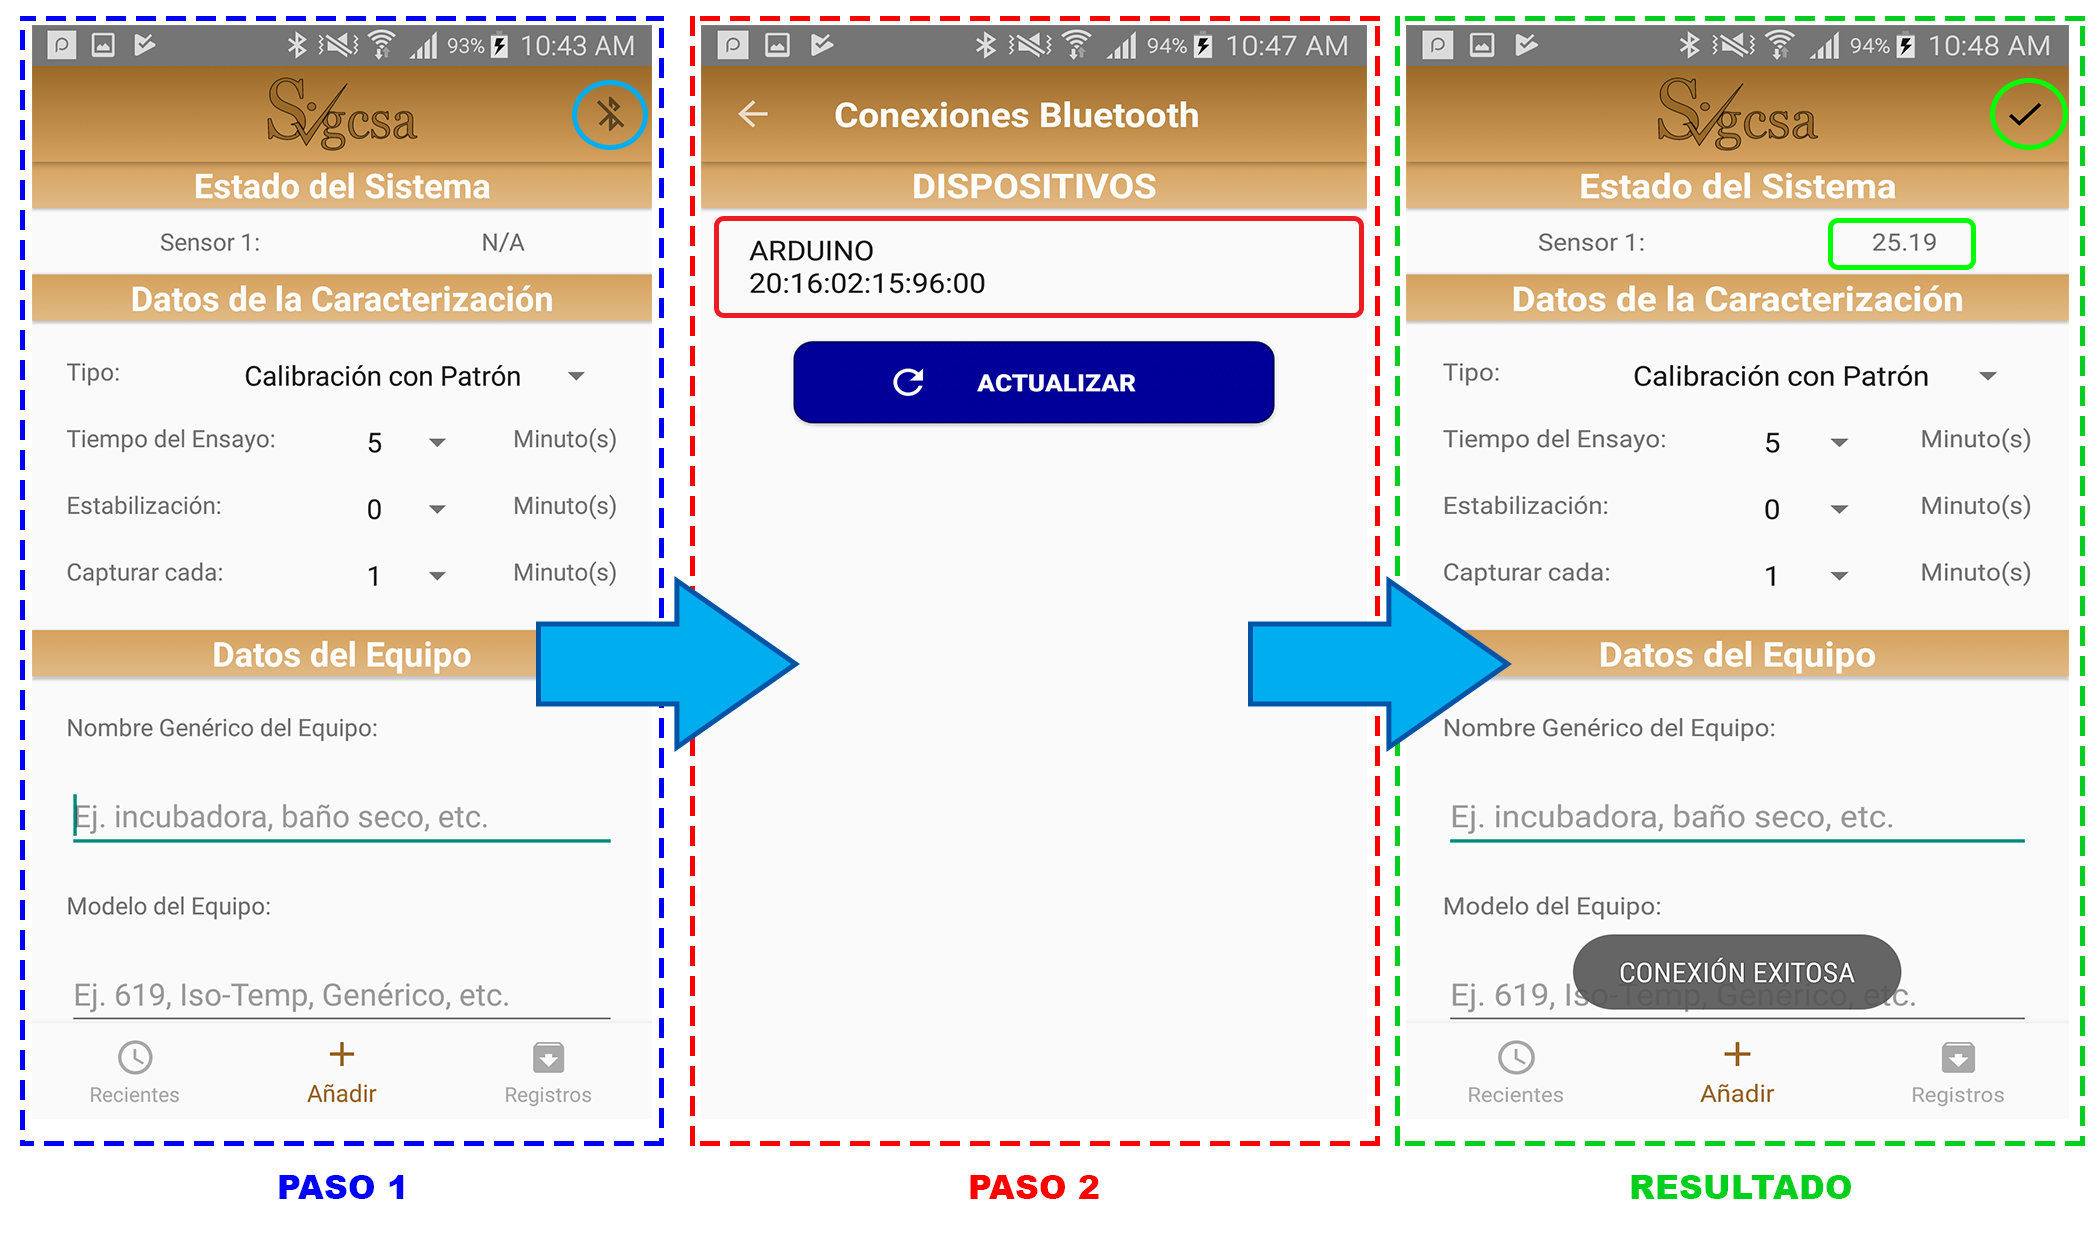
\includegraphics[width=0.8\linewidth]{interfaz13.png}
	\caption{Pasos para establecer conexión con el prototipo}
\end{figure}

\par \noindent
Si se realizó la conexión con el prototipo y la conexión se pierde se enviará un mensaje al usuario indicando lo sucedido.

\begin{figure}[H]
	\centering
	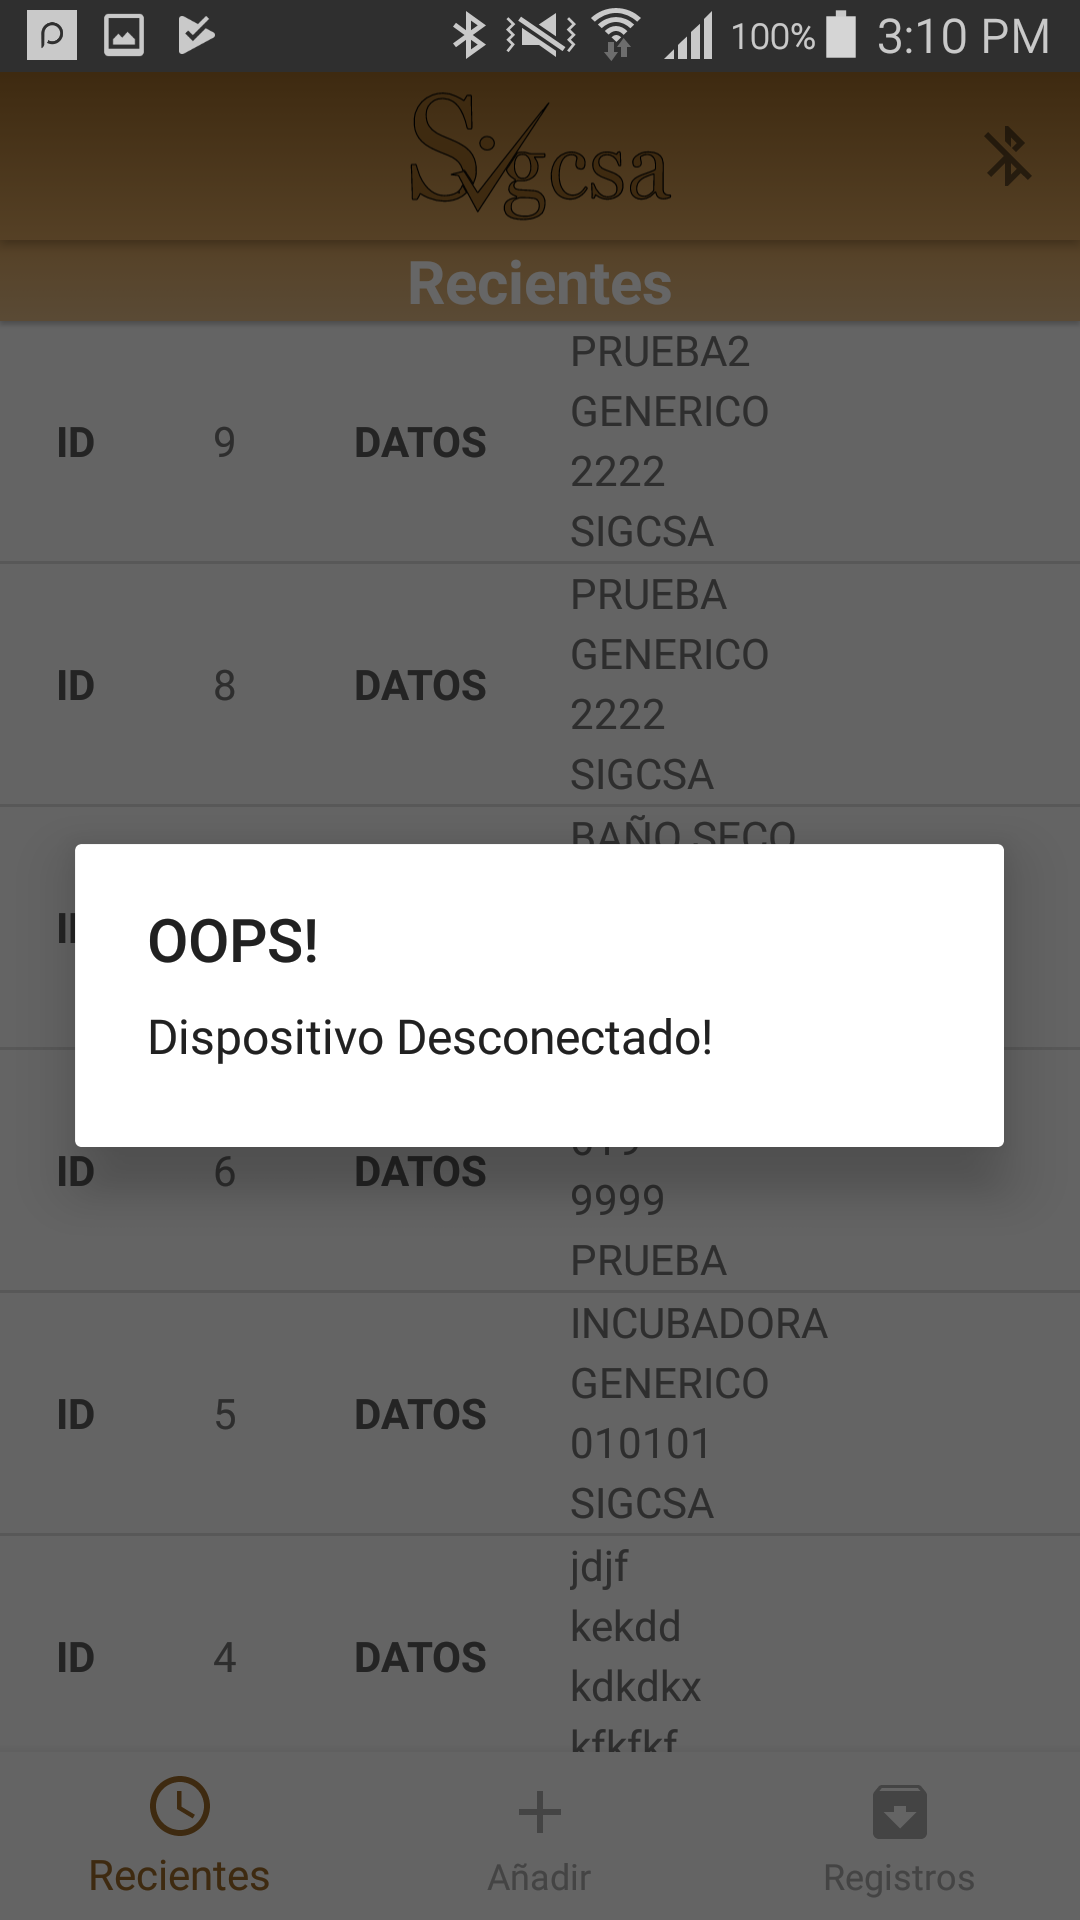
\includegraphics[width=0.3\linewidth]{interfaz14.png}
	\caption{Mensaje enviado al usuario por perdida de conexión con el prototipo}
\end{figure}

\par \noindent
Una vez establecida una conexión con el arquetipo se puede agregar un nuevo ensayo o medición.

\subsubsection{Agregar Nuevas Mediciones}

\par 
Primero hay que ubicarse en el fragmento añadir, menú inferior de la actividad principal botón "Añadir", la aplicación debe verse como en la imagen 3.14. se selecciona el tipo de ensayo, el tiempo del mismo, el tiempo de estabilización y el tiempo de captura. Luego se encuentran campos de texto para ingresar los datos del equipo a realizar el ensayo, estos campos son de texto libre. Si se llenaron todos los campos de texto y hay una comunicación activa con el dispositivo, el botón "INICIAR ENSAYO" se habilitará y cambiará a un color verde. Si se llenarón los campos de texto; pero, no hay una conexión activa con el prototipo o viceversa, el botón "INICIAR ENSAYO" no se habilitará.

\begin{figure}[H]
	\centering
	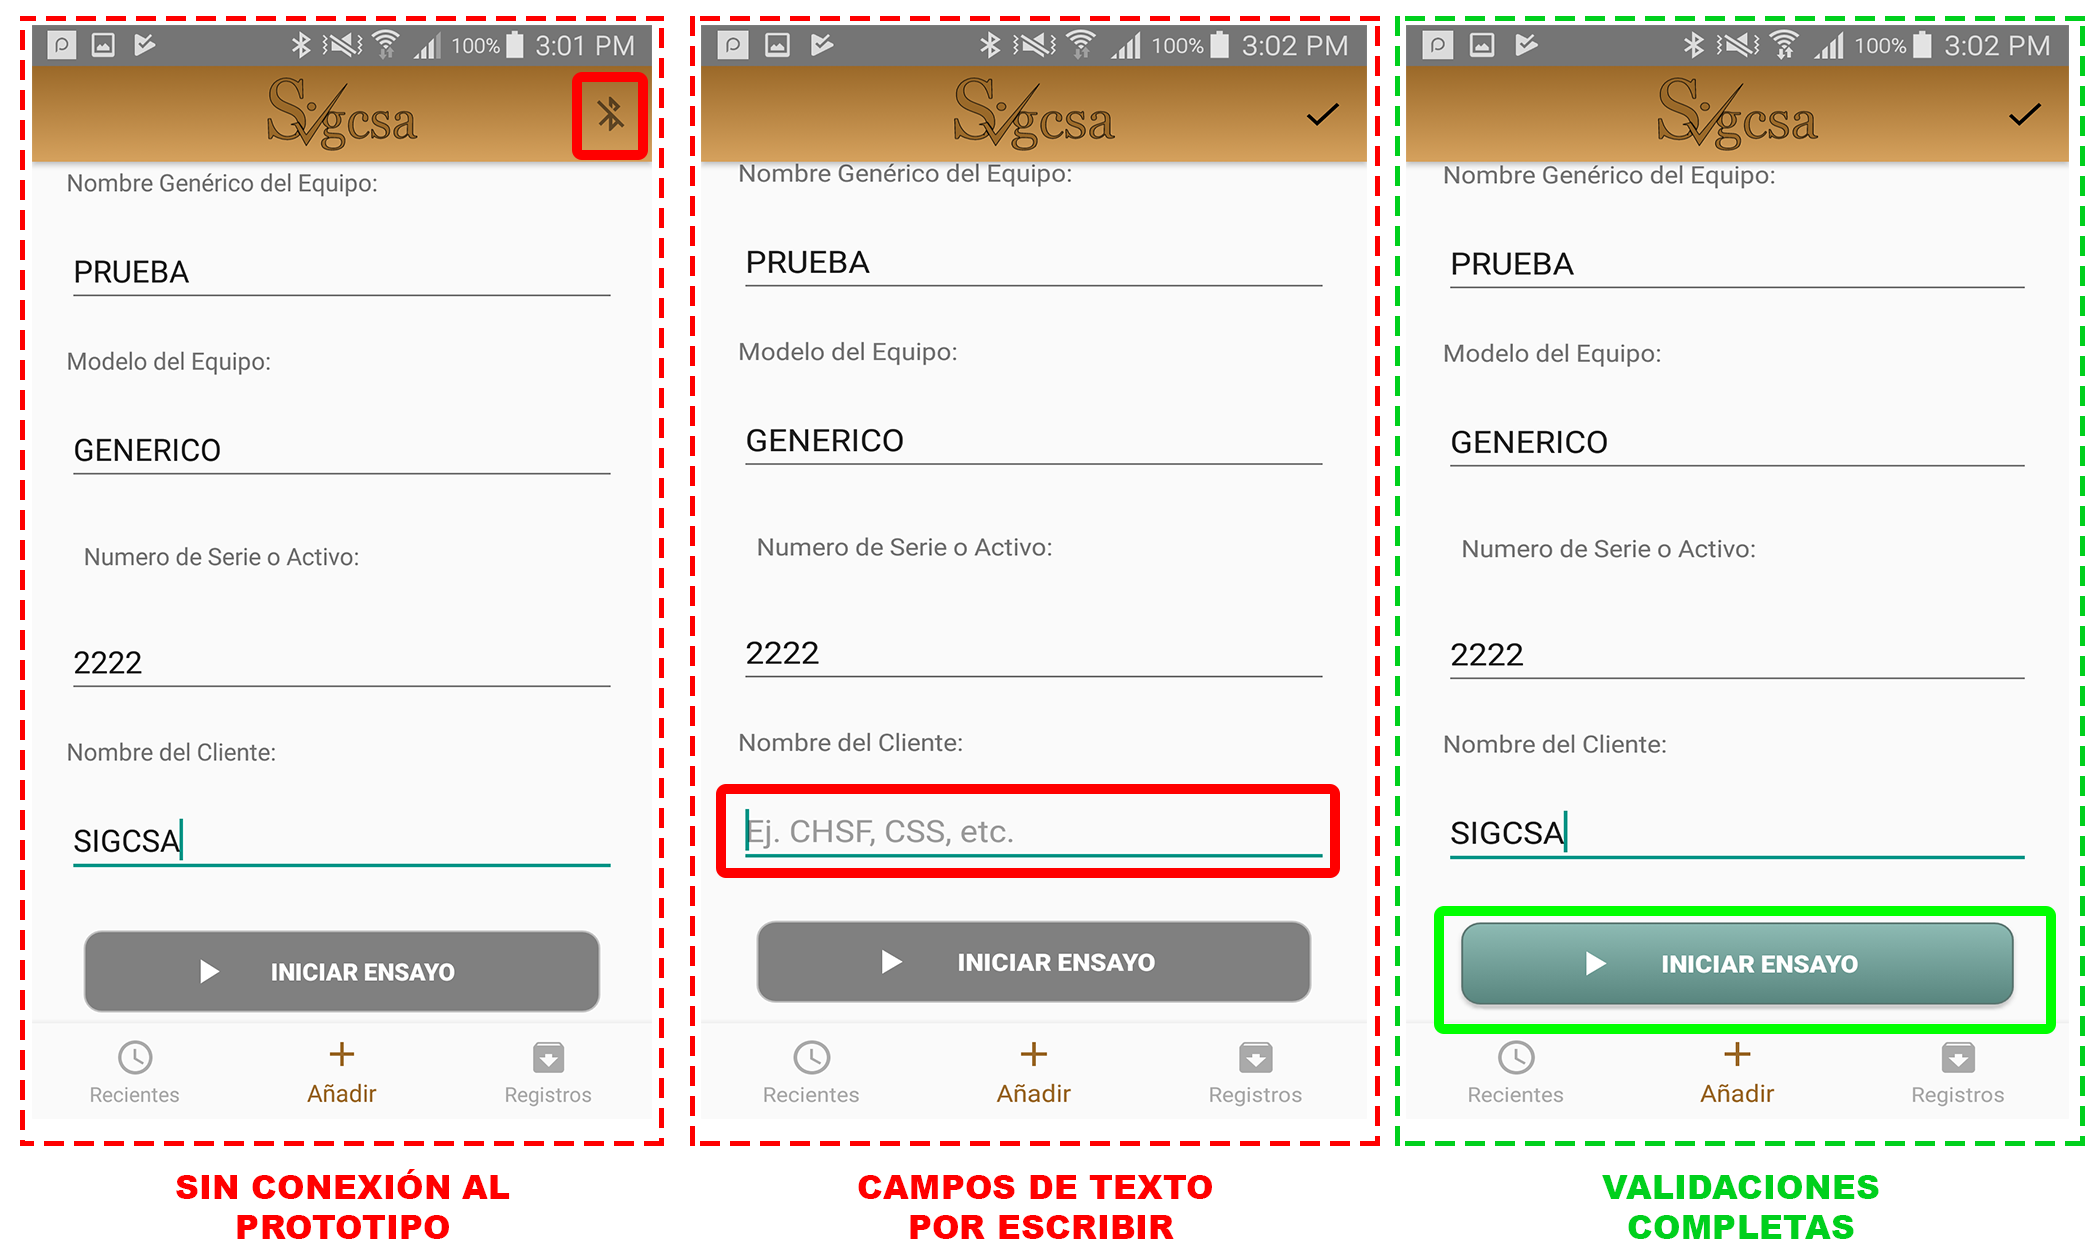
\includegraphics[width=\linewidth]{interfaz15.png}
	\caption{Validación Antes de Iniciar un Nuevo Ensayo}
\end{figure}

\par \noindent 
Una vez pulsado el botón "INICIAR ENSAYO", se deshabilitará el boton en cuestión y se habilitará el botón "CANCELAR". Además los parámetros de la medición se deshabilitarán para evitar cambios. Lo más importante es que inicia el servicio registros de mediciones el cual es el encargado de capturar los valores de los prototipos e insertarlos en la base de datos de la aplicación siguiendo los parámetros establecidos al inicio. 

\begin{figure}[H]
	\centering
	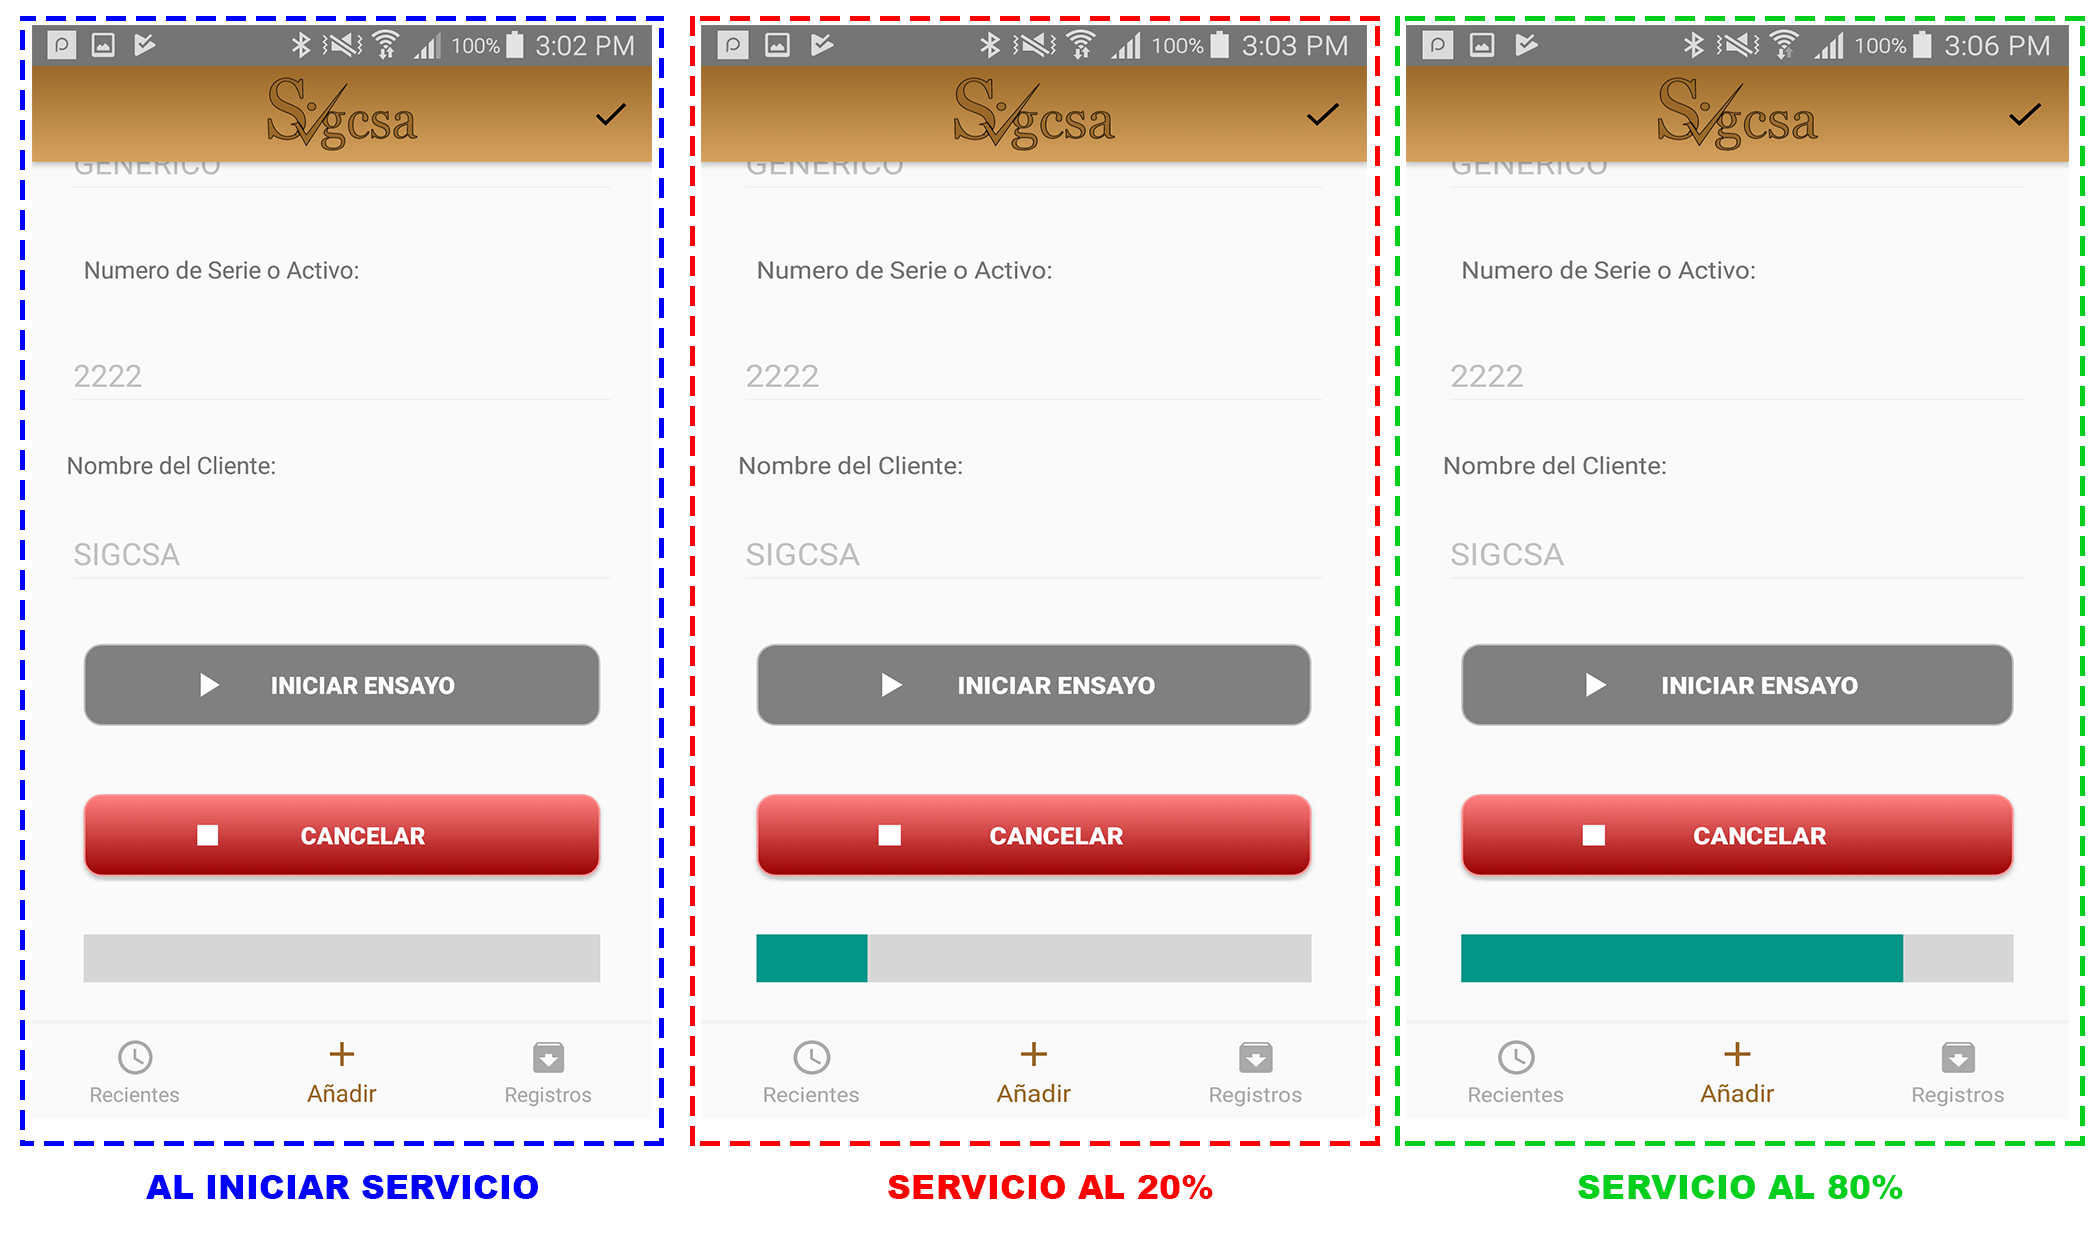
\includegraphics[width=\linewidth]{interfaz16.png}
	\caption{Proceso una vez pulsado el botón "INICIAR ENSAYO"}
\end{figure}
 
\par \noindent
Si el botón "CANCELAR" es pulsado es enviado un mensaje al servicio registros de mediciones para detener el proceso. Los valores como campos de texto y selecciones se vuelven a habilitar y el "progressbar" es reiniciado. Pulsado el botón "INICIAR SERVICIO" automáticamente se graba una fila en la base de datos. Si el servicio finaliza correctamente los valores de los campos de texto se limpian y queda el ingresa en la base de datos como "COMPLETADO". 

\par \noindent
Otro punto importante es que como el servicio registro de mediciones y servicio bluetooth de la aplicación se ejecutan en segundo plano esto quiere decir que mientras la aplicación no sea borrada de memoria. Se puede ir a otra aplicación como por ejemplo: WhatsApp, Correo, YouTube, etc. y el programa se seguirá ejecutando. Para uno se ejecutará según desee el usuario 5 minutos o una hora; mientras que, el otro se ejecuta hasta que se pierda conexión del prototipo o que se deshabilite el bluetooth del teléfono.

\par \noindent
Una vez ejecutado un ensayo hay que asegurarse que la base de datos se haya actualizado correctamente; para poder consultar las mediciones de temperatura después.

\subsubsection{Consultar una Medición Realizada Recientemente}

\par 
Para consultar una medición realizada recientemente basta solo con ubicarse en la actividad principal y seleccionar el botón "Recientes". Cada vez que se regrese al fragmento recientes, se consulta a la base de datos de la aplicación y se retornan los últimas 10 mediciones o ensayos realizados. La aplicación debe verse como en la imagen 3.11 donde se encuentra una lista de mediciones cada una con su respectiva información y número de registro (ID). Al seleccionar un elemento de la lista se desplegará más información de la medición como en la imagen 3.19. En ella se puede acceder a las mediciones de temperatura de cada sonda de manera individual con sus respectivas características como en la imagen 3.20.

\begin{figure}[H]
	\centering
	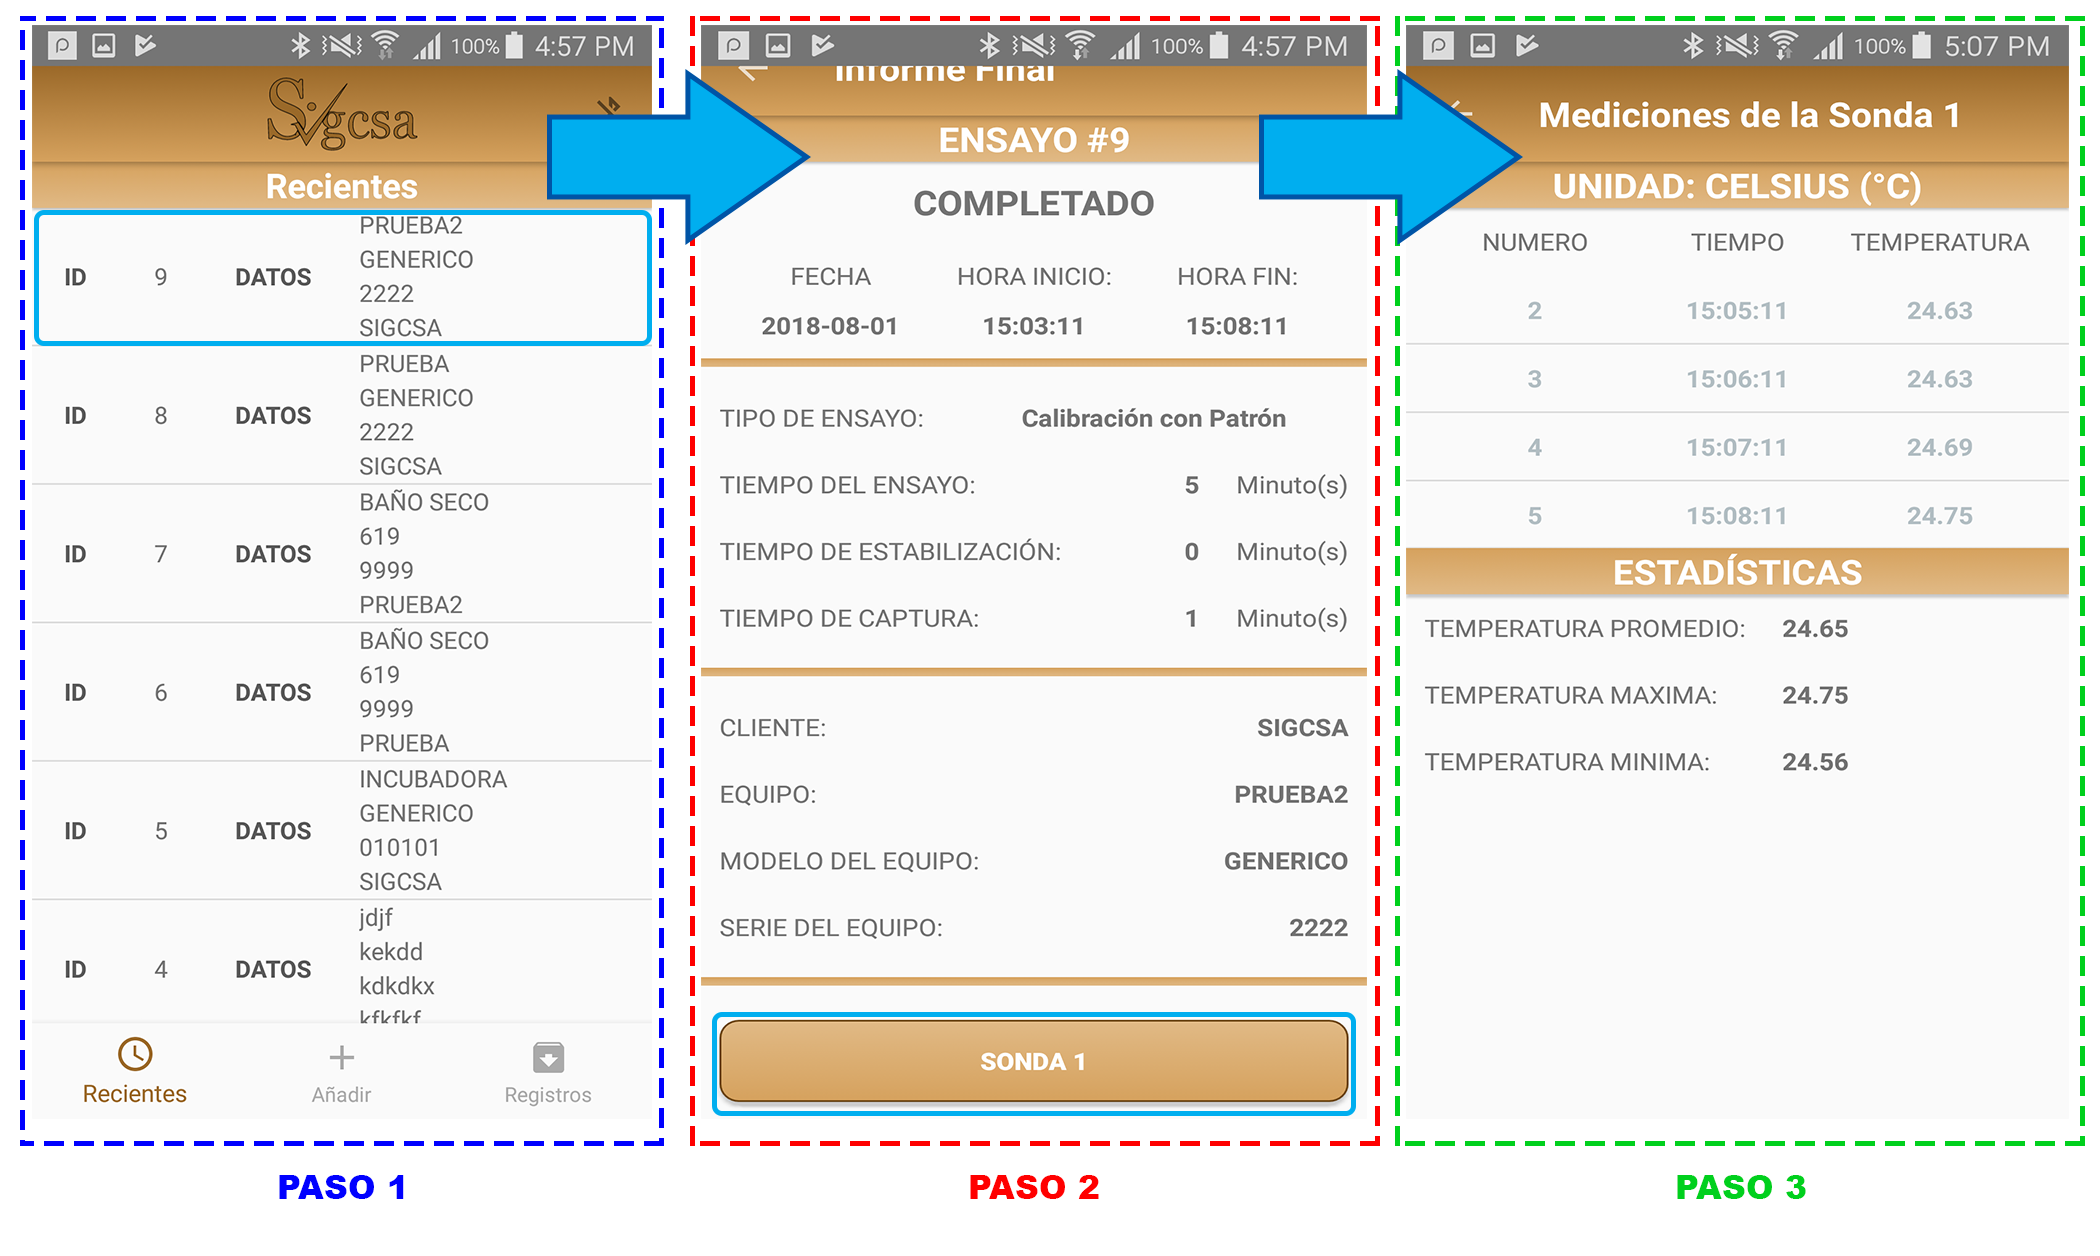
\includegraphics[width=\linewidth]{interfaz17.png}
	\caption{Proceso para consultar temperatura de una respectiva sonda en un ensayo}
\end{figure}

\par \noindent
Siempre es posible regresar al paso anterior utilizando el botón en la esquina superior izquierda o presionando la tecla de regreso del teléfono. Por último como se consulta un ensayo en un intervalo de fechas predeterminadas. 

\clearpage

\subsubsection{Consultar una Medición Realizada en una Fecha Específica}

\par 
Para consultar una medición o ensayo de una fecha específica o en un intervalo de fecha solamente hay que ubicarse en el fragmento registros, actividad principal seleccionar botón registros. La aplicación debe verse como en la imagen 3.16. Se seleciona uno de los campos con el texto "N/A" y se eligen las fechas deseadas, uno es para la fecha inicio la otra es para la fecha fin y se presiona el botón buscar. De encontrarse resultados se desplegarán en un formato de lista idéntico al formato del fragmento recientes y el proceso para consultar la información es igual al proceso anterior.

\begin{figure}[H]
	\centering
	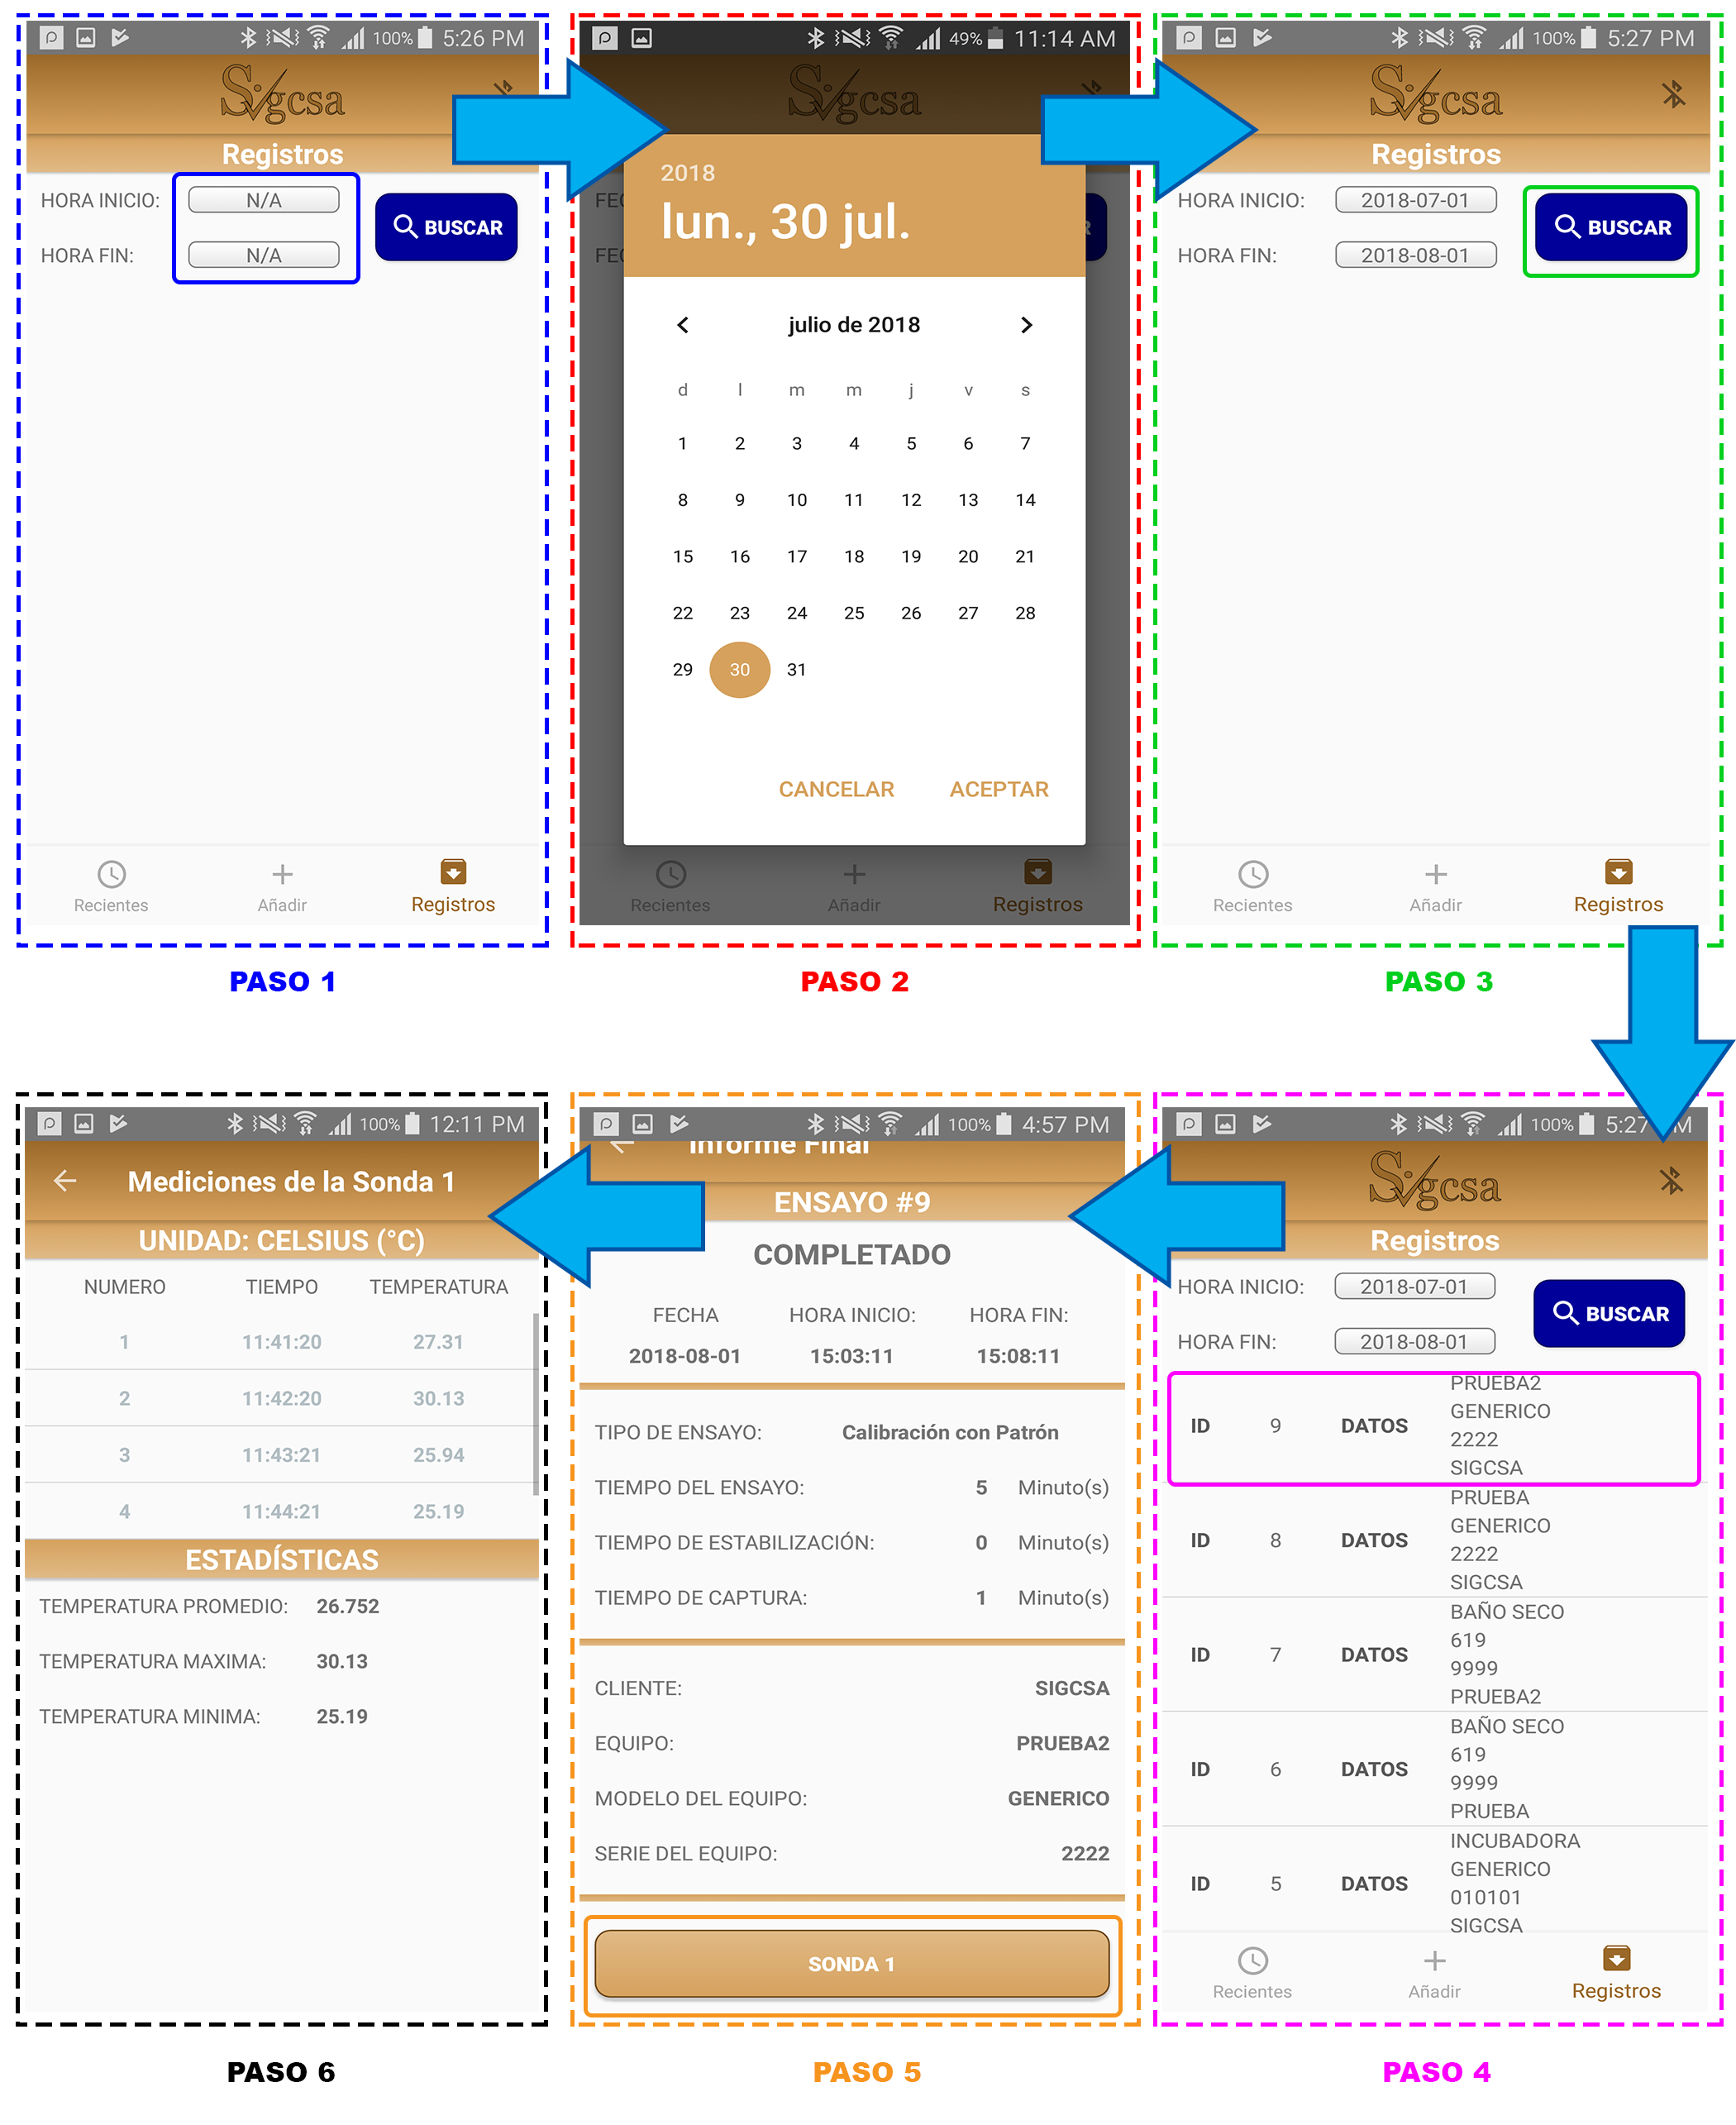
\includegraphics[width=0.8\linewidth]{interfaz18.png}
	\caption{Proceso para consultar temperatura de una respectiva sonda en un ensayo en un intervalo de fechas}
\end{figure}

\par \noindent
Se tiene conocimiento de las interfaces que se encuentran en la aplicación y como utilizarlas; sin embargo, no se sabe la parte técnica. Cuando se presionan ciertos botones se hacen llamadas a servicios que se ejecutaran en el segundo plano pero ¿Como funcionan estos servicios?


\subsection{Servicios en Segundo Plano}

\par 
Según la documentación oficial de Android un servicio es un punto de entrada de propósito general para mantener una aplicación ejecutándose en segundo plano por todo tipo de razones. Es un componente que se ejecuta en segundo plano para realizar operaciones de larga ejecución o para realizar trabajos en procesos remotos. Un servicio no proporciona una interfaz de usuario. Por ejemplo, un servicio puede reproducir música en segundo plano mientras el usuario está en una aplicación diferente, o puede obtener datos a través de la red sin bloquear la interacción del usuario con una actividad. Otro componente, como una actividad, puede iniciar el servicio y permitir que se ejecute o se vincule con él para interactuar con él. En realidad, hay dos servicios semánticos muy distintos que le dicen al sistema cómo administrar una aplicación: los servicios iniciados le dicen al sistema que los mantenga funcionando hasta que se complete su trabajo. Esto podría ser para sincronizar algunos datos en segundo plano o reproducir música incluso después de que el usuario abandone la aplicación.\cite{androidapp}

\par \noindent
Mencionado anteriormente nuestra aplicación cuenta con dos servicios que se ejecutan en el segundo plano uno para mantener una comunicación bluetooth entre el prototipo y la aplicación. El otro para capturar las medidas de temperatura de nuestro prototipo. 

\subsubsection{Servicio Bluetooth}

\par \noindent
Cuando se está desarrollando una aplicación en Android; ya se encuentran disponible un paquete genérico para utilizar la antena bluetooth de la mayoría del smartphone. Este paquete "android.bluetooth" contiene clases para ciertas tareas individuales para el manejo de la antena. Las clases utilizadas del paquete "android.bluetooth" son:

\begin{itemize}
	\item BluetoothAdapter
	
	\item BluetoothDevice
	
	\item BluetoothSocket
\end{itemize}

\par \noindent
Las clases anteriormente mencionadas contienen funciones para obtener información de un dispositivo bluetooth que se encuentra conectado a nuestro smartphone. Otra función importante es que nos permiten instanciar objetos con información del dispositivo al que nos encontramos conectado, objetos con información de nuestra antena e información del "socket" si hay una conexión activa. 

\par \noindent
Un socket es un objeto de software que actúa como un punto final que establece un enlace bidireccional de comunicación de red entre un lado del servidor y un programa del lado del cliente.\cite{socket}

\par \noindent
En Java, lenguaje utilizado en el desarrollo de aplicaciones en Android, las clases de socket representan la comunicación entre los programas del cliente y del servidor. Las clases de socket manejan la comunicación del lado del cliente, y las clases de socket del servidor manejan la comunicación del lado del servidor.\cite{socket}

\par \noindent
Teniendo claro lo necesario para desarrollar el servicio, debemos desarrollar 3 clases que se comunicaran entre sí.

\begin{itemize}
	\item BTAsynk: Es la clase que se encargara de establecer una comunicación con el dispositivo bluetooth deseado. Se encarga de guardar información de la conexión en memoria y valida si la conexión es exitosa.
	
	\item BTsocketHandler: Es una clase publica pero sus atributos y métodos son estáticos. Esto significa que los valores asignados y retornados de esta clase son compartidas en todas las instancias de ella. Esto es importante porque garantiza que no hallan fugas de memoria en nuestra aplicación. En ella se guarda la información obtenida por BTAsynk para ser utilizadas después.
	
	\item BTservice: Una vez BTAsynk ha establecido una conexión correctamente, esta clase hace llamados a atributos de BTsocketHandler para validar que seguimos conectados al dispositivo bluetooth y envía esa información del segundo plano al primer plano de nuestra aplicación. Esto es gracias a que BTservice hereda atributos y métodos de la clase IntentService.
	
\end{itemize}

\par \noindent
Según la documentación oficial de Android la clase IntentService es una clase base para servicios que manejan solicitudes asíncronas (expresadas como Intents) ha pedido. Los clientes envían solicitudes a través de llamadas Context.startService (Intent); el servicio se inicia según sea necesario, maneja cada intención a su vez utilizando un hilo de trabajo, y se detiene cuando se queda sin trabajo.\cite{intentservice}

\par \noindent
Este patrón de "procesador de cola de trabajo" se usa comúnmente para descargar tareas del hilo principal de una aplicación. La clase IntentService existe para simplificar este patrón y cuidar la mecánica de la aplicación. \cite{intentservice}

\par \noindent
En conclusión la clase BTAsynk es la encargada de establecer una comunicación bluetooth con el prototipo. Si la conexión es exitosa entonces BTAsynk envía información del dispositivo y socket activo a la clase BTSocketHandler y por último inicia la clase BTService. La clase BTService entra en un ciclo while donde transformará las medidas de temperatura enviadas por el prototipo a un objeto JSON y el objeto JSON es enviado a la clase BTsocketHandler. Adicional durante este ciclo BTService estará enviando un mensaje a la actividad principal indicando que la conexión esta activa. En la actividad principal mientras BTService se encuentre enviando el mensaje, el icono del botón bluetooth será un gancho como en la imagen 4.24. Cuando el mensaje ya no sea recibido entonces enviara la notificación al usuario que la conexión con el prototipo se a caído como en la imagen 4.22. Los códigos para las clases anteriormente mencionadas se encuentran en el Anexo 2.

\subsubsection{Servicio de Registro de Temperatura}

\par 
El Servicio de Registro de Temperatura es el encargado de convertir el objeto JSON de la clase BTSocketHandler a consultas de SQL para guardarlas en la base de datos SQLite de nuestro dispositivo.

\par \noindent
SQLite es una librería en proceso que implementa un motor de base de datos SQL transaccional independiente, sin servidor y de configuración cero. El código para SQLite es de dominio público y, por lo tanto, es gratuito para cualquier uso, comercial o privado. SQLite es la base de datos más implementada del mundo con más aplicaciones de las que podemos contar, incluidos varios proyectos de alto perfil.SQLite es un motor de base de datos SQL incorporado. A diferencia de la mayoría de las otras bases de datos SQL, SQLite no tiene un proceso de servidor por separado. SQLite lee y escribe directamente en archivos de disco ordinarios. Una base de datos SQL completa con múltiples tablas, índices, disparadores y vistas, está contenida en un solo archivo de disco.\cite{sqlite}

\par \noindent
Anteriormente se había mencionado que la clase BTSocketHandler es estática para que sus instancias compartan la misma información. Esto es esencial debido a que para realizar inserciones en la base de datos en tiempo real es necesario que el servicio bluetooth y el servicio registro de temperatura se encuentren trabajando simultáneamente en el segundo plano, sin afectar el rendimiento de la aplicación y la clase BTSocketHandler actuando como un puente entre ambos servicios.

\par \noindent
En Android no hay clases para crear o manejar una base de datos; sin embargo, el paquete "android.database" nos brinda las clases necesarias para nosotros desarrollar una sola clase que se encargue del manejo de la base de datos de nuestra aplicación. Vamos a necesitar del paquete "android.database" las siguientes clases:

\begin{itemize}
	
	\item android.database.Cursor
	
	\item android.database.sqlite.SQLiteDatabase
	
	\item android.database.sqlite.SQLiteOpenHelper
	
\end{itemize} 

\par \noindent
Con estas clases podemos desarrollar una clase que es la utilizaremos en nuestra aplicación para crear la base de datos y realizar las diferentes consultas e inserciones a la base de datos. El Código de esta clase llamada "DatabaseHelper" se encuentra en el Anexo 3.

\par \noindent
Para iniciar el servicio basta con presionar el botón "INICIAR ENSAYO" del fragmento añadir. Automáticamente el fragmento añadir envía los datos de su interfaz como los campos de textos y los parámetros seleccionados por el usuario. Luego el servicio obtiene esos valores y creamos una instancia de la clase "DatabaseHelper" la cual si el fichero de la base de datos no se ha creado la crea automáticamente. 

\par \noindent
Los valores del fragmento añadir son ordenados para realizar la primera inserción en la base de datos. Si esta primera inserción es válida entonces preguntamos el valor del tiempo de estabilización seleccionado en el fragmento añadir. Si el valor es diferente de 0 entonces utilizamos el comando "SystemClock.sleep" para detener la ejecución del servicio por el tiempo que se solicitó.

\par \noindent
Luego dependiendo del tiempo de tipo de ensayo (Isotermo 1, Isotermo 2 o Calibración con Patrón) entonces seleccionamos la tabla y los valores a insertar. Una vez seleccionados el servicio entra en un ciclo for donde se estará llamando el objeto JSON de la clase BTsocketHandler para realizar las inserciones correspondientes, el ciclo for se ejecutará por el tiempo que estipulo el usuario y cada vez que se realice un ciclo se envía el porcentaje del ensayo hasta el momento al "progressbar" del fragmento añadir.

\par \noindent
Por último se valida que el usuario no presiono el botón cancelar y se actualiza la primera inserción realizada en el servicio.

\par \noindent
Ambos servicios interactúan entre sí para crear validaciones al usuario y poder actualizar la base de datos correctamente. Sin embargo es necesario saber la estructura de la base de datos; ya que, no solamente es utilizada por los servicios sino también por el usuario al momento de consultar la información capturada. 

\clearpage


\subsection{Base de Datos SQLite}

\par \noindent
La base de datos SQLite definida en la sección es donde se guardan todas las medidas de temperatura realizadas por nuestro prototipo. El hecho de ser simplemente un fichero en nuestro smartphone lo hace versatil y efeciente para una base de datos local. 


\par \noindent
Por base de datos local hacemos entender que la información se mantendra en la memoria del smartphone que se este utilizando. SQLite se base en una base de datos SQL; por lo que, implementaremos una base de datos relacional. 

\begin{figure}[H]
	\centering
	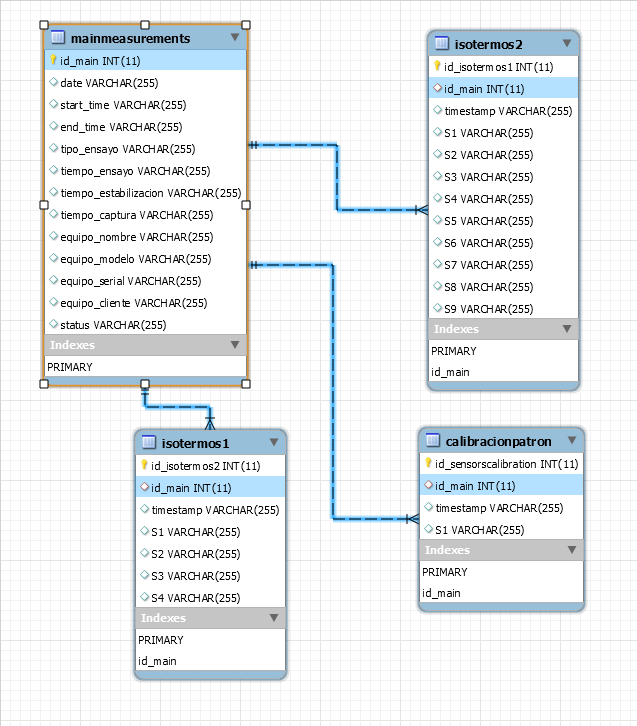
\includegraphics[width=0.8\linewidth]{db1.png}
	\caption{Estructura de la Base de Datos}
\end{figure}

\clearpage

\par \noindent
La tabla principal vendría siendo "mainmeasurements" donde se toman los datos del equipo y parámetros del ensayo. Mientras que las otra tablas con los nombres de los tipos de ensayo son donde se guardan las medidas de temperatura. Estas tablas estan relacionadas a la tabla principal, pero no entre ellas.
